\documentclass[USenglish]{article}
\setlength\parindent{0pt}
%%%%%%%%%%%%%%
\usepackage{fullpage}
\usepackage{amsmath,amsfonts,amsthm,amssymb}
\usepackage{color,xcolor}
\usepackage{ifpdf}
\usepackage{psfrag}
\usepackage{graphicx,graphics}
\usepackage{hhtensor}
\usepackage{comment}
\usepackage[small]{caption}
\usepackage{subcaption}

\usepackage{xparse}
\usepackage{bigints}

\usepackage{pgfplots}
\usepackage{tikz}
\usetikzlibrary{positioning,calc}
\pgfplotsset{compat=1.18}



\usepackage{url}
\usepackage{hyperref}
\usepackage{todonotes}
\usepackage{cleveref}
\usepackage{ulem} \normalem
% ------------------------------------------
\newtheorem{theorem}{Theorem}[section]
\newtheorem{corollary}[theorem]{Corollary}
\newtheorem{lemma}[theorem]{Lemma}
\newtheorem{proposition}[theorem]{Proposition}
\newtheorem{remark}[theorem]{Remark}
\newtheorem{definition}[theorem]{Definition}
\newtheorem{example}[theorem]{Example}
\newtheorem{assumption}[theorem]{Assumption}
\newtheorem{conclusion}[theorem]{Conclusion}

\usepackage{cancel}
\usepackage{algorithm,algorithmic}
\usepackage{enumitem}

\usepackage{mathtools, mathrsfs}
\usepackage{bbm}
\usepackage{fancybox}
\usepackage[nottoc]{tocbibind}
\usepackage{float}



\newcommand{\R}{\mathbb R}
\newcommand{\Z}{\mathbb Z}
\newcommand{\N}{\mathbb N}
\newcommand{\C}{\mathbb C}
\newcommand{\Q}{\mathbb Q}
\newcommand{\K}{\mathbb K}
\renewcommand{\L}{\mathcal L}
\newcommand{\I}{\mathcal I}
\newcommand{\PP}{\mathbb P}
\newcommand{\TT}{\mathcal{T}}
\newcommand{\normal}{\mathbf{N}}

\renewcommand{\SS}{\mathcal{S}}
\newcommand{\KK}{\mathcal{K}}
\newcommand{\EE}{\mathcal{E}}

% ---- Notation Philipp
\newcommand{\ww}[1]{\underline{#1}}
\renewcommand{\div}{\operatorname{div}}
\newcommand{\est}[1]{\left\langle#1\right\rangle}
\newcommand{\bU}{\mathbf{U}}
\newcommand{\bH}{\mathbf{H}}
\newcommand{\dd}{\mathrm{d}}
\newcommand{\bV}{\mathbf{V}}
\newcommand{\mean}[1]{\overline{#1}}
\newcommand{\bbfh}{{\mathbf {f}^h}}
\newcommand{\Ol}{\mathcal{O}}
\newcommand{\WW}{\mathrm{W}}
\newcommand{\LL}{\mathcal{L}}
\newcommand{\II}{\hat{I}_0}
\newcommand{\1}{\begin{pmatrix}
		1\\
		1
\end{pmatrix}}


\newcommand\norm[1]{\left\lVert#1\right\rVert}

\newcommand{\tp}{t^{n+1}}
\newcommand{\tn}{t^{n}}


\renewcommand{\vec}[1]{\ww{#1}}
\NewDocumentCommand{\mat}{mo}{%
	\IfValueTF{#2}{%
		\underline{\underline{#1}}{#2}
	}{%
		\underline{\underline{#1}}\,
	}%
}
%Davide

\usepackage{bbm}
\def\bbc{\underline{\boldsymbol{\alpha}}}
\def\bc{\boldsymbol{\alpha}}
\def\bbu{\underline{\boldsymbol{u}}}
\def\bu{\boldsymbol{u}}
\def\bbv{\underline{\boldsymbol{v}}}
\def\bv{\boldsymbol{v}}
\def\bbw{\underline{\boldsymbol{w}}}
\def\bw{\boldsymbol{w}}
\def\br{\boldsymbol{r}}
\def\bd{\mathbf{d}}
\def\bbd{\underline{\mathbf{d}}}
\def\bphi{\underline{\phi}}
\def\M{\underline{\underline{\mathrm{M}}}}
\def\S{\underline{\underline{\mathrm{S}}}}

\def\TMM{\textsc{TMM}}
\def\DeC{\textsc{DeC}}
\def\ADER{\textsc{ADER}}
\def\sDeC{\textsc{sDeC}}
\def\eq{\textsc{EQ}}
\def\GLB{\textsc{GLB}}

\def\NODES{\textsc{NODES}}


%Colors 
\definecolor{darkspringgreen}{rgb}{0., 0.55, 0.3}
\definecolor{dartmouthgreen}{rgb}{0.05, 0.5, 0.06}
\definecolor{etonblue}{rgb}{0.59, 0.78, 0.64}
\definecolor{airforceblue}{rgb}{0., 0.4, 0.66}
\definecolor{arylideyellow}{rgb}{0.91, 0.84, 0.42}
\definecolor{emerald}{rgb}{0.31, 0.78, 0.47}
\definecolor{uclagold}{rgb}{1.0, 0.7, 0.0}
\definecolor{cadmiumorange}{rgb}{0.93, 0.53, 0.18}


\newtheorem{prop}{Proposition}




%Shorten for Entropy function
\newcommand{\Ucof}[2]{U_{(#1)}^{(#2)}}
\newcommand{\Vcof}[2]{\bv_{(#1)}^{(#2),T}}
\newcommand{\ecof}[2]{\eta_{(#1)}^{(#2)}}

% Corrections
\newcommand{\rev}[1]{#1}%{\textcolor{red}{#1}}
\newcommand{\PO}[1]{{\color{blue}#1}}
\newcommand{\DT}[1]{{\color{darkspringgreen}#1}}
\newcommand{\LP}[1]{{\color{brown}#1}}
\newcommand{\DTT}[1]{{\color{darkspringgreen}#1}}
\newcommand{\revMA}[1]{#1}%{\textcolor{darkspringgreen}{#1}}
%%%%%%%%%%%%%%%
\hypersetup{
	pdftitle={IMEX DeC and ADER},
	pdfauthor={P. \"Offner, L. Petri and D. Torlo},
	pdfpagemode=UseOutlines,
	linkbordercolor=0 0 0,
	linkcolor=red,
	citecolor=blue,
	colorlinks=true,
	bookmarks = true
}



\makeatletter
\def\namedlabel#1#2{\begingroup
	#2%
	\def\@currentlabel{#2}%
	\phantomsection\label{#1}\endgroup
}
\makeatother

% Sets running headers as well as PDF title and authors
%\headers{ADER and DeC for Advection-Diffusion}{ P. \"Offner, A. Thomann, and D. Torlo}

% Title. If the supplement option is on, then "Supplementary Material"
% is automatically inserted before the title.
\title{Analysis for Implicit and Implicit-Explicit ADER and DeC Methods for Ordinary Differential Equations, Advection-Diffusion and Advection-Dispersion Equations}

%Authors: full names plus addresses.
\author{
	Philipp \"Offner\thanks{Institute of Mathematics, Johannes Gutenberg University, Mainz, Germany, (\email{poeffner@uni-mainz.de}, \orcid{0000-0002-1367-1917})
	} 
	\and 
	Louis Petri\thanks{Institute of Mathematics, Johannes Gutenberg University, Mainz, Germany, (\email{lpetri01@uni-mainz.de}), } 
	\and 
	Davide Torlo\thanks{Dipartimento di Matematica Guido Castelnuovo, Università di Roma La Sapienza,  Roma, Italy, (\email{davide.torlo@uniroma1.it})} 
}



\usepackage{amsopn}


\begin{document}
	\title{Analysis for Implicit and Implicit-Explicit ADER and DeC Methods for Ordinary Differential Equations, Advection-Diffusion and Advection-Dispersion Equations:\\ Extra material}
	
	\author{Philipp \"Offner\thanks{Institute of Mathematics, Johannes Gutenberg University, Mainz, and Institute of Numerical Analysis,  TU Clausthal, Clausthal-Zellerfeld, Germany, mail@philippoeffner.de},
	Louis Petri\thanks{Institute of Mathematics, Johannes Gutenberg University, Mainz, Germany, lpetri01@uni-mainz.de },  
	Davide Torlo\thanks{Dipartimento di Matematica Guido Castelnuovo, Università di Roma La Sapienza,  Roma, Italy, davide.torlo@uniroma1.it}
	}
	\date{}
	\maketitle
	
	%\keywords{test} 
%	\begin{abstract}
%		%In this paper, we develop implicit and implicit-explicit ADER and DeC methods 
%within the framework of the two-operators DeC and we study their stability as ODE solvers and in the context of linear PDE.
%We reformulate the methods as Runge-Kutta schemes to investigate their stability, discovering  that the methods strongly differ (from A-stable to bounded stability regions) according to the choice of order, method and quadrature nodes, differently from their explicit counterparts. 
%When applied to advection-diffusion and advection-dispersion equations (with finite difference spatial discretization), the von Neumann stability analysis shows that they are stable under CFL-like conditions and for the advection-diffusion equation even under a spatial-independent restriction. 
%We provide precise bounds for such coefficients and suggestion on which scheme is adequate in different problems.
\PO{

In this manuscript, we present the development of implicit and implicit-explicit ADER and DeC methodologies within the DeC framework using the two-operators formulation, with a focus on their stability analysis both as solvers for ordinary differential equations (ODEs) and within the context of linear partial differential equations (PDEs).
To analyze their stability, we reinterpret these methods as Runge-Kutta schemes and uncover significant variations in stability behavior, ranging from A-stable to bounded stability regions, depending on the chosen order, method, and quadrature nodes. 
This differentiation contrasts with their explicit counterparts.
When applied to advection-diffusion and advection-dispersion equations employing finite difference spatial discretization, the von Neumann stability analysis demonstrates stability under CFL-like conditions. 
Particularly noteworthy is the stability maintenance observed for the advection-diffusion equation, even under spatial-independent constraints.
Furthermore, we establish precise boundaries for relevant coefficients and provide suggestions regarding the suitability of specific schemes for different problem.
}




	
%	\end{abstract}
%	\tableofcontents
	\section{Introduction} 
\label{sec:introduction} 
Many systems of time-dependent differential equations can be separated into multiple parts that differ in their stiffness. For such systems, using implicit-explicit (IMEX) time-marching methods \cite{pareschi2000implicit} is of paramount importance to guarantee stability and accuracy in many applications.

At the same time, high-order time-marching methods are sought for their efficiency and to match with the spatial discretization order in time-dependent partial differential equations (PDEs). Explicit high-order ADER and deferred correction (DeC) methods, due to their automatic construction, emerge as suitable alternatives to the traditional Runge-Kutta (RK) methods and have been extensively explored in various studies.
The explicit DeC method, introduced by Dutt et al. \cite{dutt2000dec} and then reinterpreted by Abgrall \cite{abgrall2017dec}, is an explicit, arbitrarily high-order method for ODEs. Further extensions of DeC, including implicit, semi-implicit and modified Patankar versions, are available in the literature \cite{christlieb2010integral,minion2003dec,offner2019arbitrary,abgrall2022relaxation,layton2004conservative,speck2015multi}. 
The ADER method was originally developed for hyperbolic systems exploiting the Cauchy-Kovalevskaya theorem \cite{ADERHistorical2, ADERHistorical1,titarev2002ader}, then reinterpreted  as a space-time discontinuous Galerkin (DG) method, which is solved through a fixed-point iteration procedure \cite{ADERModern,zbMATH07627644,dumbser2007FVStiff,boscheri2014direct,micalizzi2023efficient,veiga2023improving,Han_Veiga_2021}.

%In this work, we describe and analyze the implicit and IMEX version of ADER and DeC, both as ODE solvers and in the context of advection--diffusion or advection--dispersion PDEs. The description follows previous studies \cite{Han_Veiga_2021, minion2003dec, abgrall2018asymptotic}, where an IMEX description of DeC and ADER was already provided, but we extend the analysis to all possible methods, using different quadrature points and order of accuracy. Moreover, we study their IMEX stability in the spirit of \cite{Hundsdorfer,liotta2000central, minion2003dec}, noting large differences across the methods, from bounded stability areas to A-stable ones. This is in contrast with the behavior of the explicit versions.


In this research, we present an detailed investigation of both implicit and IMEX versions of ADER and DeC, investigating their efficacy as solvers for ordinary differential equations (ODEs) and in the context of linear  advection-diffusion or advection-dispersion partial differential equations (PDEs).
Building upon prior work \cite{Han_Veiga_2021, minion2003dec, abgrall2018asymptotic, dumbser2007FVStiff}, which has explored IMEX descriptions of DeC and ADER, we expand our analysis to encompass the most used methods, employing varying quadrature points and levels of accuracy. Additionally, we explore their IMEX stability following the approach of previous studies \cite{Hundsdorfer,liotta2000central, minion2003dec}, uncovering notable discrepancies among them, ranging from bounded stability regions to A-stable ones. This diverges significantly from the behavior observed in explicit versions \cite{Han_Veiga_2021}.

Extending our investigation to the PDE case and inspired by  \cite{TanChenShu_ImEx_Stability}, 
%For the PDE case, inspired by \cite{TanChenShu_ImEx_Stability}, 
we conduct a von Neumann analysis for the presented IMEX time discretizations, paired with finite difference spatial discretizations of corresponding accuracy levels.
We find that the stability regions are bounded by CFL-type conditions as well as simple conditions on $\Delta t$ for the advection--diffusion case. 
%\PO{Emphasize this significant point: The CFL-type bounds remain invariant regardless of the spatial discretization method applied.}
% that do not involve the spatial discretization. 
 
% For the advection--dispersion, the analysis gives less clear results and only in few cases some conditions only dependent on spatial discretization. 
%All these findings are in agreement with the ODE stability regions found above.

The analysis of advection-dispersion presents less definitive outcomes, with only a few cases indicating conditions solely influenced by spatial discretization. However, these findings align with the stability regions observed in the ODE case.

%The paper is organized as follows. 
%In Section~\ref{sec:dec} and \ref{sec:ader}, we introduce the implicit and IMEX DeC and ADER methods, respectively, and we embed them into the RK framework. 
%We also provide some theoretical stability results for the pure implicit ADER method. In Section~\ref{sec:convergence}, we prove the high order accuracy of the implicit and IMEX ADER and DeC methods. In Section~\ref{sec: stability_analysis_ODE}, we describe their stability regions. In Sections~\ref{sec: advection_diffusion} and \ref{sec:PDE_adv_disp}, we extend the stability analysis to the PDE case by applying our IMEX methods to advection-diffusion and advection-dispersion equations.
%In Section~\ref{sec:numerics}, we perform few numerical examples to validate the stability and convergence analysis, and in Section~\ref{sec:conclusion} we draw some conclusions.

The structure of the paper is as follows. In Sections~\ref{sec:dec} and \ref{sec:ader}, we introduce the implicit and IMEX DeC and ADER methods, respectively, and incorporate them into the RK framework. Additionally, we present theoretical stability results for the pure implicit ADER method.
In Section~\ref{sec:convergence}, we establish the high order accuracy of both the implicit and IMEX ADER and DeC methods. Following this, in Section~\ref{sec: stability_analysis_ODE}, we delineate their stability regions.
Next, in Sections~\ref{sec: advection_diffusion} and \ref{sec:PDE_adv_disp} we extend the stability analysis to the PDE scenario by applying our IMEX methods to advection-diffusion and advection-dispersion equations.
In Section~\ref{sec:numerics}, we finally present several numerical examples aimed at validating the stability and convergence analyses, while in Section~\ref{sec:conclusion} we summarize the conclusions drawn from our deep analysis. 

	
	
	\section{Numerical Stability Analysis}
	\label{sec: stability_analysis_ODE}
	In this section, we study the stability of the presented method for the linear Dahlquist equation $u' = -\lambda u$ or $u' = -\lambda_I u - \lambda_E u$ for IMEX methods. All methods can be rewritten as $u_{n+1} = R(z)u_n$ or $u_{n+1}= R(z_I,z_E)$ being $R$ stability functions and $z,z_I,z_E\in \mathbb C$. 
We will study the stability regions $\lbrace |R|\leq 1\rbrace \subset \mathbb C$ for the explicit and implicit ADER/DeC, while for the IMEX schemes we consider different approaches. 
We will use equispaced (eq) or Gauss-Lobatto (GLB) nodes as quadrature nodes.
We will numerically compute the stability regions obtained from the stability functions of ADER/DeC that are defined through their Butcher tableaux, see \cite{hairer1987solving}.
In detail, we compute on $200\times 200$ grid points with an offset of $+0.01$ from the origin for both axes to avoid singularities. 
The plot bounds are dependent on the type of scheme and their stability regions.
We decreased the offset in Figures~\ref{fig: ODE_minor_instabilitys} to a fraction of $10^{-2}$ of the largest real value displayed when zooming on small areas.

%All of the following pictures have been obtained by plugging the above described Butcher tableaux into the stability functions, using property \eqref{eq:ImExStabilityFunction} and evaluating them numerically.\\
%While the explicit cases have already been investigated in \cite{Han_Veiga_2021}, we will investigate the implicit stability regions for the first time at this point. 
%A slight extension to these results can be found in the appendix.
To distinguish the different orders, we apply different colors and line styles to the outer and inner bounds according to the legend that are plot next to each stability region plot.
%in figure~\ref{fig: legend_standard}.
%\begin{figure}[!h]
%	\centering
%		\begin{minipage}[t]{0.4\textwidth}\centering
%			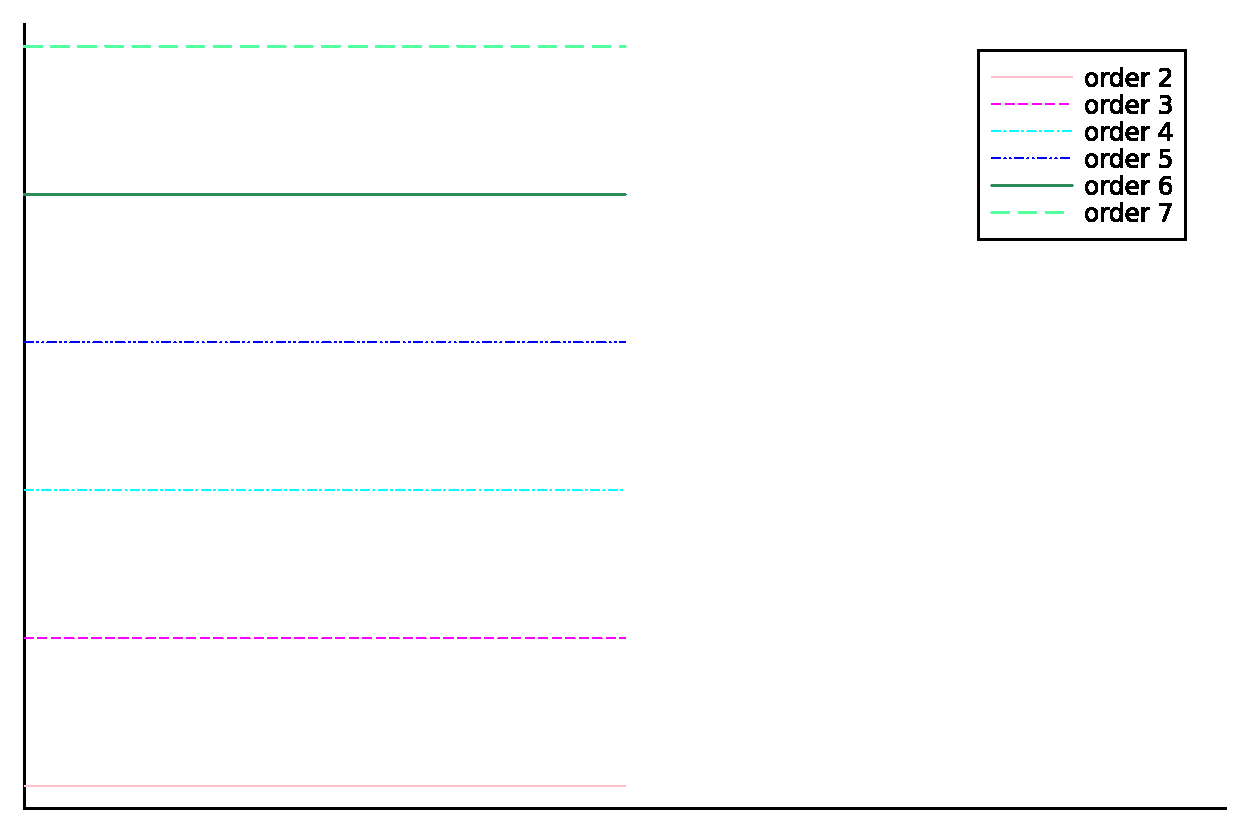
\includegraphics[height=0.4\textwidth, trim={469 280 30 23}, clip]{pdf/odepics/colors_a-d_new_2-7.pdf}
%			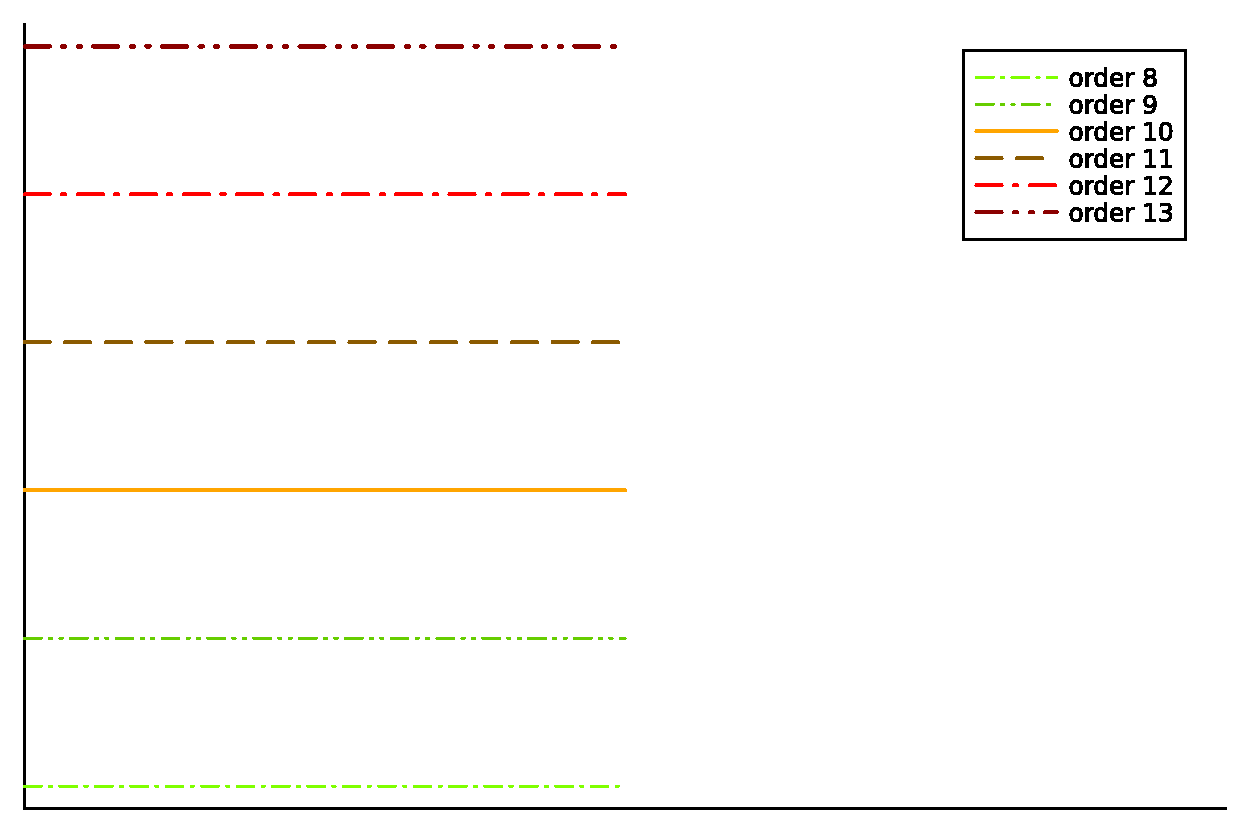
\includegraphics[height=0.4\textwidth, trim={461 280 30 23}, clip]{pdf/odepics/colors_a-d_new_8-13.pdf}
%		\end{minipage}
%		\caption{Legend for the classic RK and the IMEX stability regions}
%	\label{fig: legend_standard}
%\end{figure}
\subsection{Stability analysis of explicit schemes}\label{sec:stability_explicit}
In figure~\ref{fig: ODEEX} (left), we show the results obtained in \cite{Han_Veiga_2021}, extended up to order 13. It was pointed out, that the regions of the explicit ADER and DeC coincide and that they are independent of the chosen interpolation nodes. Here, we just display them once. We can highlight the growth of stability by increasing the order of the respective method. 
\begin{figure}
	\centering
	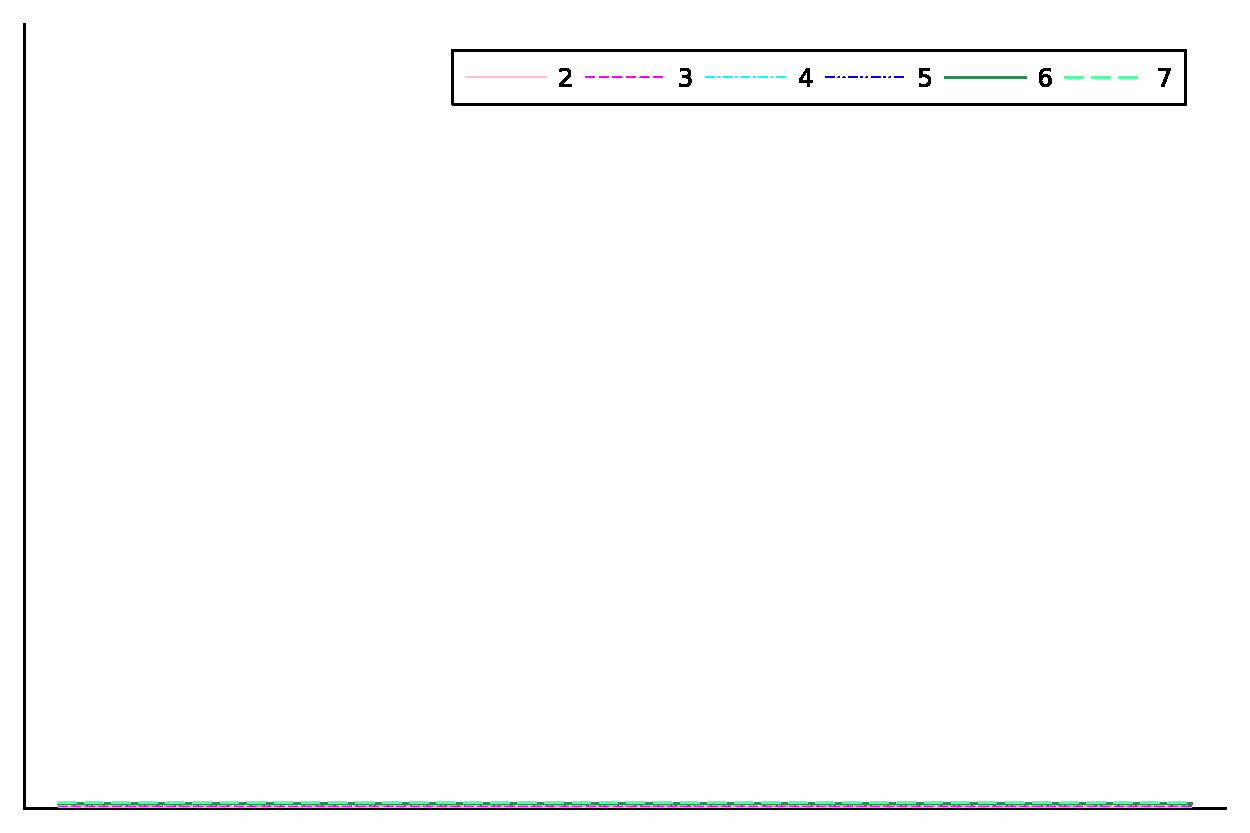
\includegraphics[width=0.465\textwidth,trim={215 340 32 22}, clip]{pdf/odepics/colors_a-d_new_horiz_2-7_no_order.pdf}\!\!
	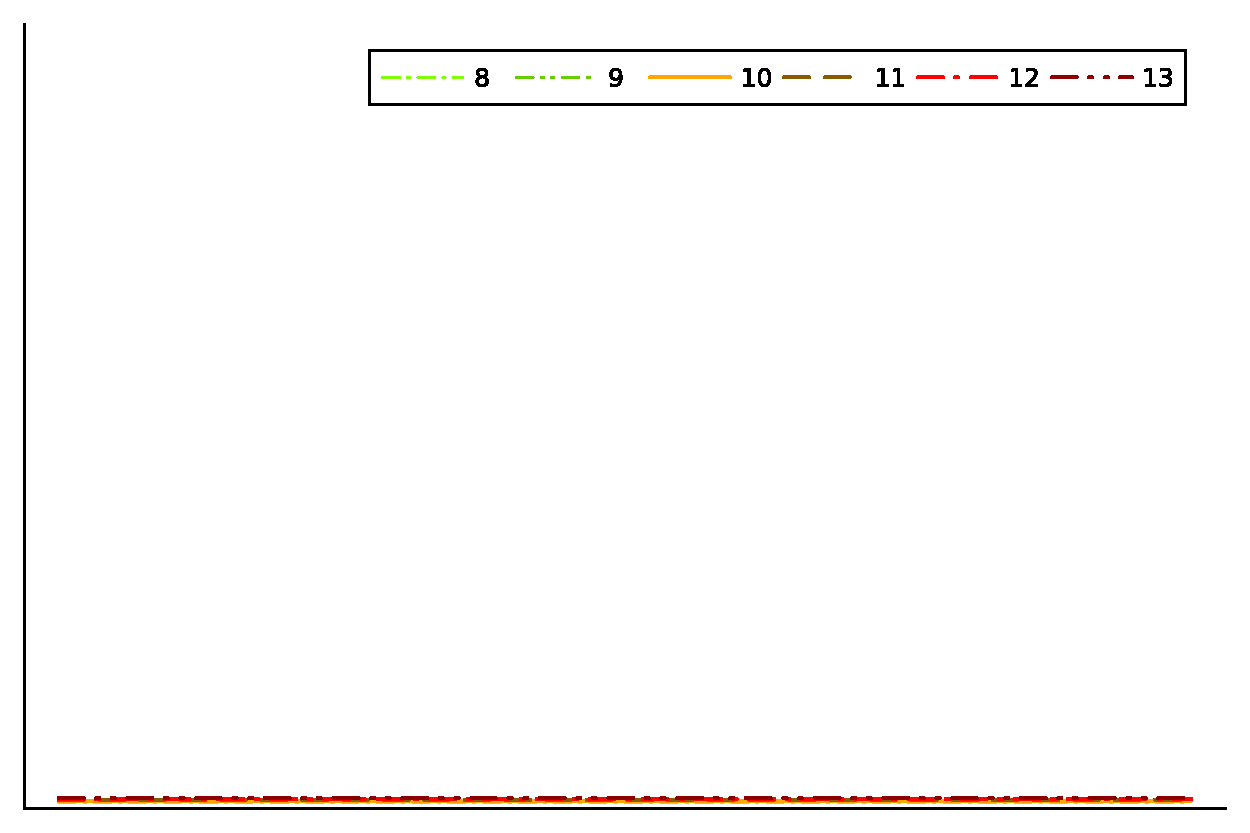
\includegraphics[width=0.515\textwidth,trim={179 340 30 22}, clip]{pdf/odepics/colors_a-d_new_horiz_8-13_no_order.pdf}\\
	\begin{minipage}[t]{0.32\textwidth}
		\centering
		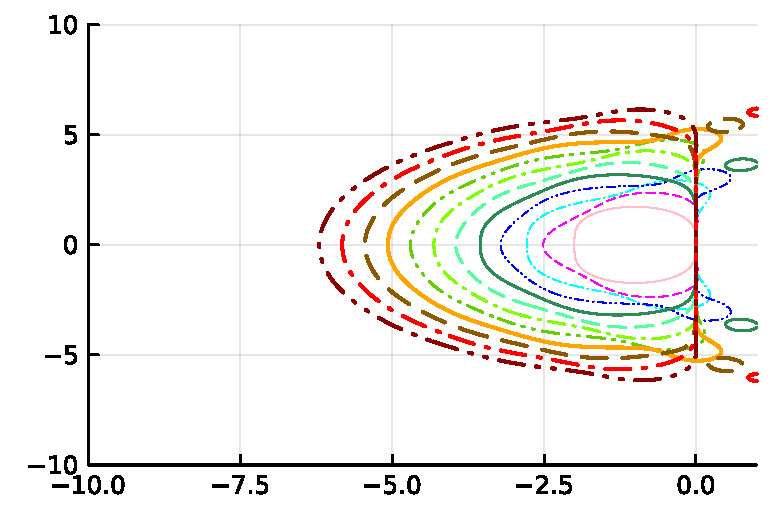
\includegraphics[width=\textwidth]{pdf/odepics/DeC_GLB_ord13.pdf}\\
		DeC/ADER eq/GLB
	\end{minipage}
	\begin{minipage}[t]{0.32\textwidth}
		\centering
		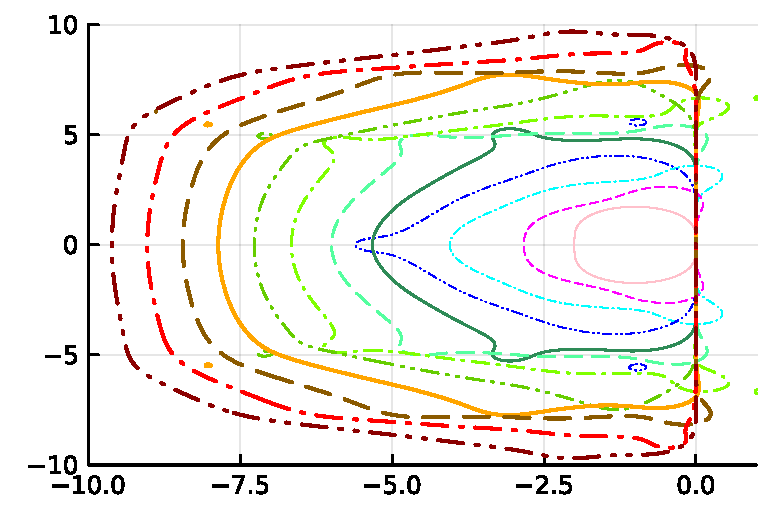
\includegraphics[width=\textwidth]{pdf/odepics/sDeC_eq_ord13.pdf}\\
		sDeC eq
	\end{minipage}
	\begin{minipage}[t]{0.32\textwidth}
		\centering
		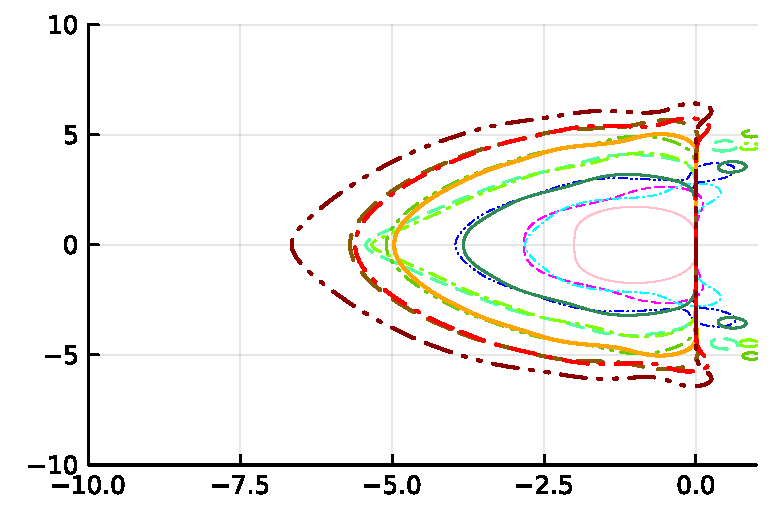
\includegraphics[width=\textwidth]{pdf/odepics/sDeC_GLB_ord13.pdf}\\
		sDeC GLB
	\end{minipage}
	\caption{Stability regions for the explicit ADER and DeC methods with GLB or equispaced nodes for orders 2 to 13 (left), sDeC equispaced (center) and sDeC GLB (right).}
	\label{fig: ODEEX}
\end{figure}

Furthermore, we want to take a look at the explicit sDeC, whose stability regions can be observed in figure~\ref{fig: ODEEX} (center and right). 
This method differs not only from the ADER and DeC, but also from sDeC with different nodes. The qualitative shape is still similar to the others, but it is just remarkable that the sDeC methods with equispaced interpolation points have respectively larger stability regions.
\subsection{Implicit schemes}
In the following, we plot the contour lines of the bounds of the stability regions of various implicit methods. We start from ImDeC (left) and ImADER (right) schemes with equispaced nodes (top) and GLB nodes (bottom) in Figure~\ref{fig: ODEIMDeCADER} up to order 13. 
Clearly, all these stability regions are unbounded, but they are not all A-stable, as we will see soon. Moreover, we can observe a great variability changing the scheme or the nodes, in opposition to the explicit case \cite{Han_Veiga_2021}. In most of the cases, ImADER have larger stability regions than ImDeC.
\begin{figure}
	\centering
	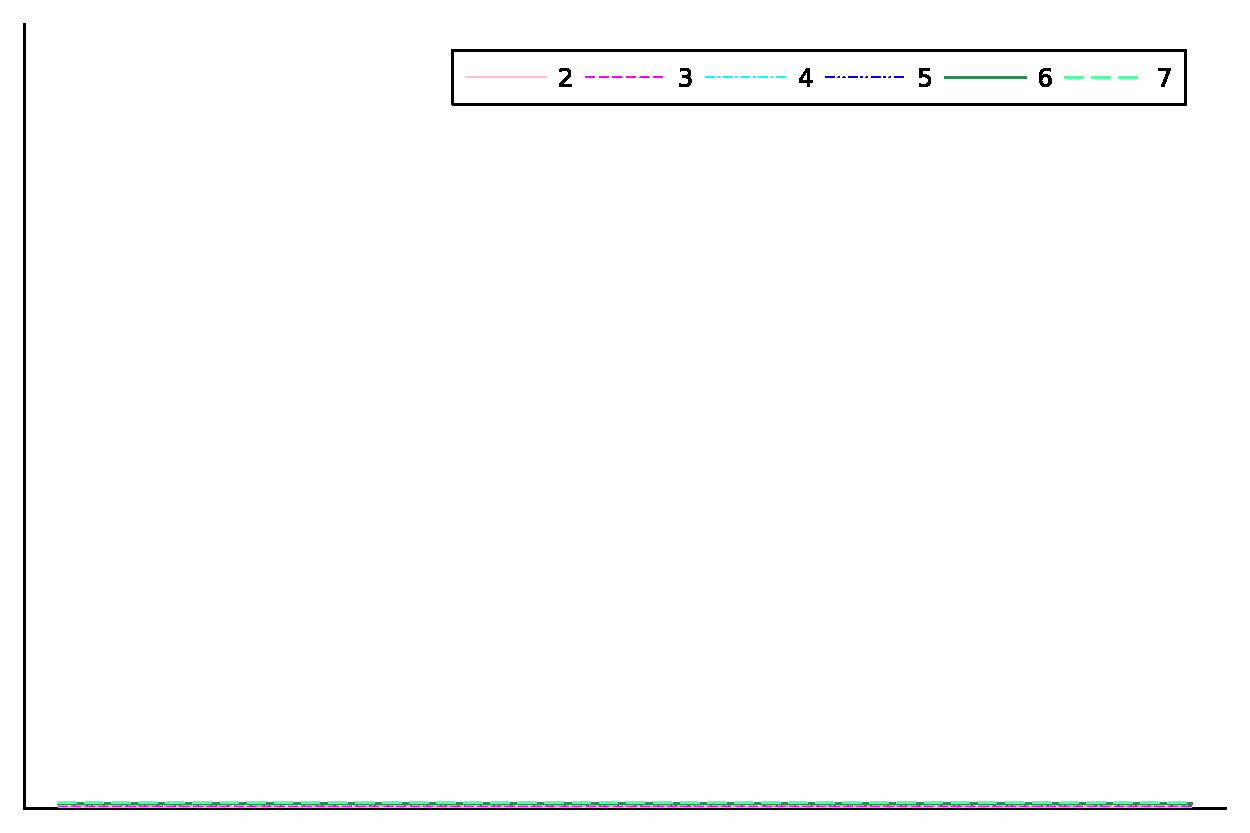
\includegraphics[width=0.465\textwidth,trim={215 340 32 22}, clip]{pdf/odepics/colors_a-d_new_horiz_2-7_no_order.pdf}\!\!
	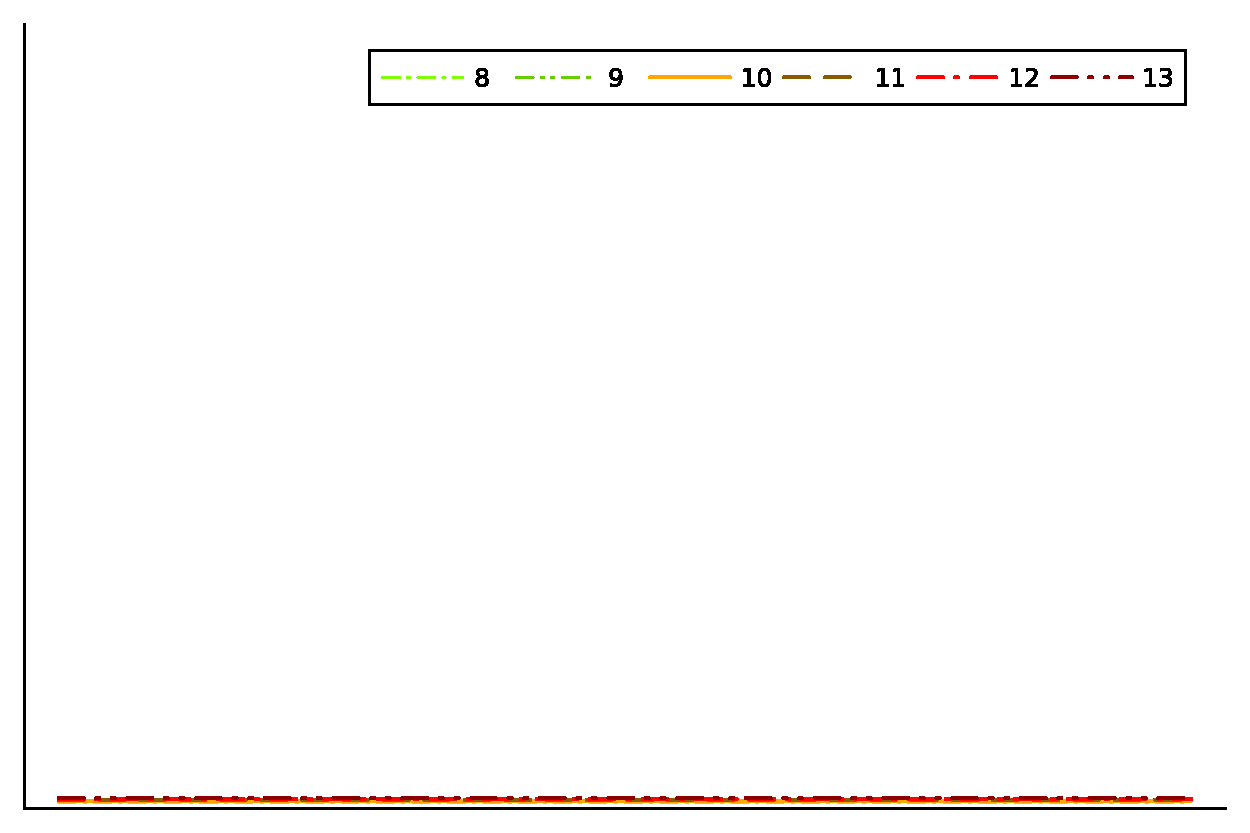
\includegraphics[width=0.515\textwidth,trim={179 340 30 22}, clip]{pdf/odepics/colors_a-d_new_horiz_8-13_no_order.pdf}\\
	\begin{minipage}[t]{0.32\textwidth}
		\centering
		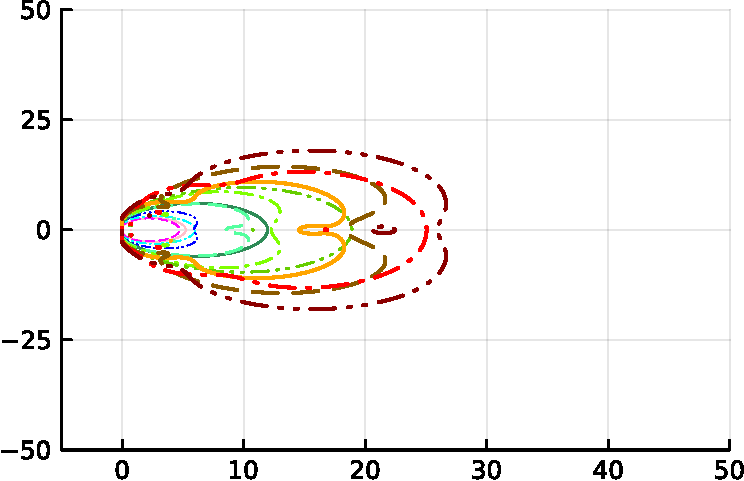
\includegraphics[width=\textwidth, trim={0 0 0 0}, clip]{pdf/odepics/IMDeC_eq_ord13-crop.pdf}\\
		ImDeC eq
	\end{minipage}
	\begin{minipage}[t]{0.32\textwidth}
		\centering
	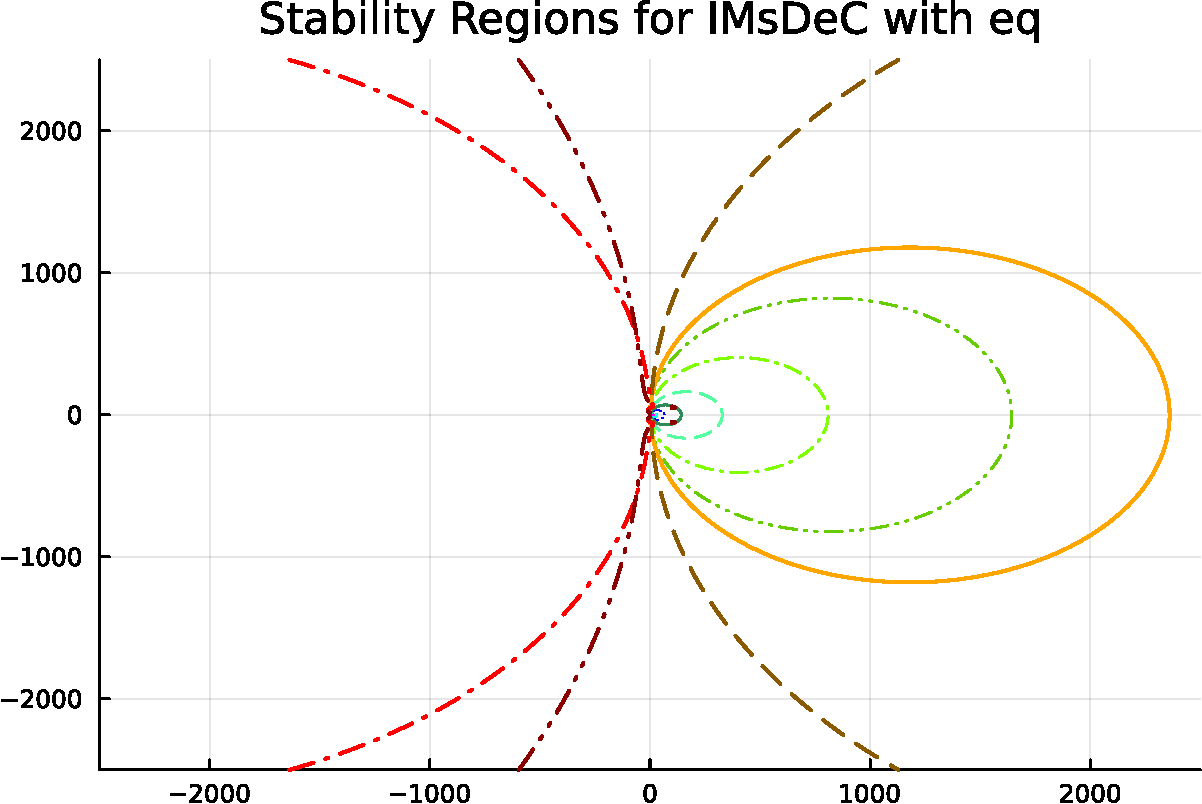
\includegraphics[width=\textwidth, trim={0 0 0 0}, clip]{pdf/odepics/IMsDeC_eq_ord13-crop.pdf}\\
	ImsDeC eq
	\end{minipage}
	\begin{minipage}[t]{0.32\textwidth}
		\centering
		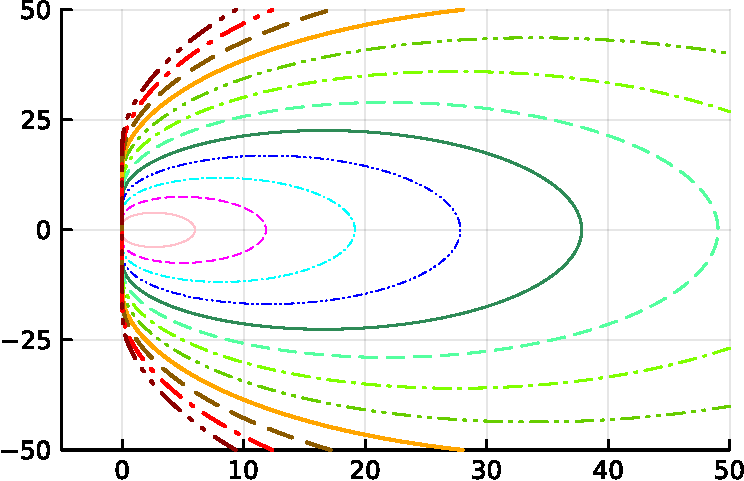
\includegraphics[width=\textwidth, trim={0 0 0 0}, clip]{pdf/odepics/IMADER_eq_ord13-crop.pdf}\\
		ImADER eq
	\end{minipage}\\
	\begin{minipage}[t]{0.32\textwidth}
		\centering
		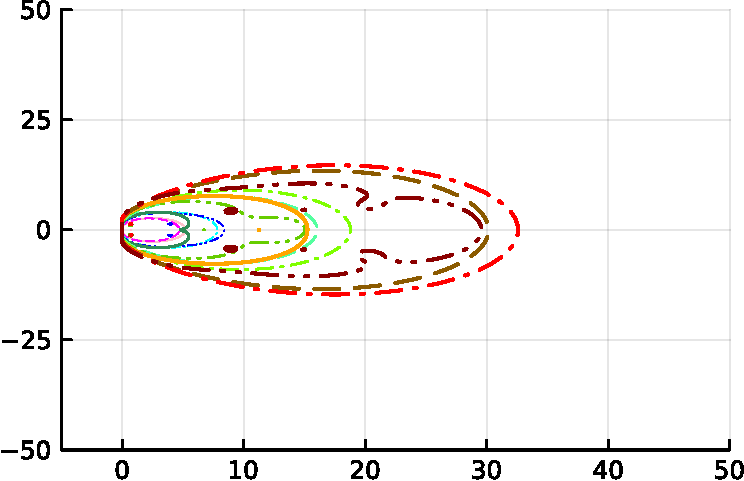
\includegraphics[width=\textwidth, trim={0 0 0 0}, clip]{pdf/odepics/IMDeC_GLB_ord13-crop.pdf}\\
		ImDeC GLB
	\end{minipage}
	\begin{minipage}[t]{0.32\textwidth}
		\centering
	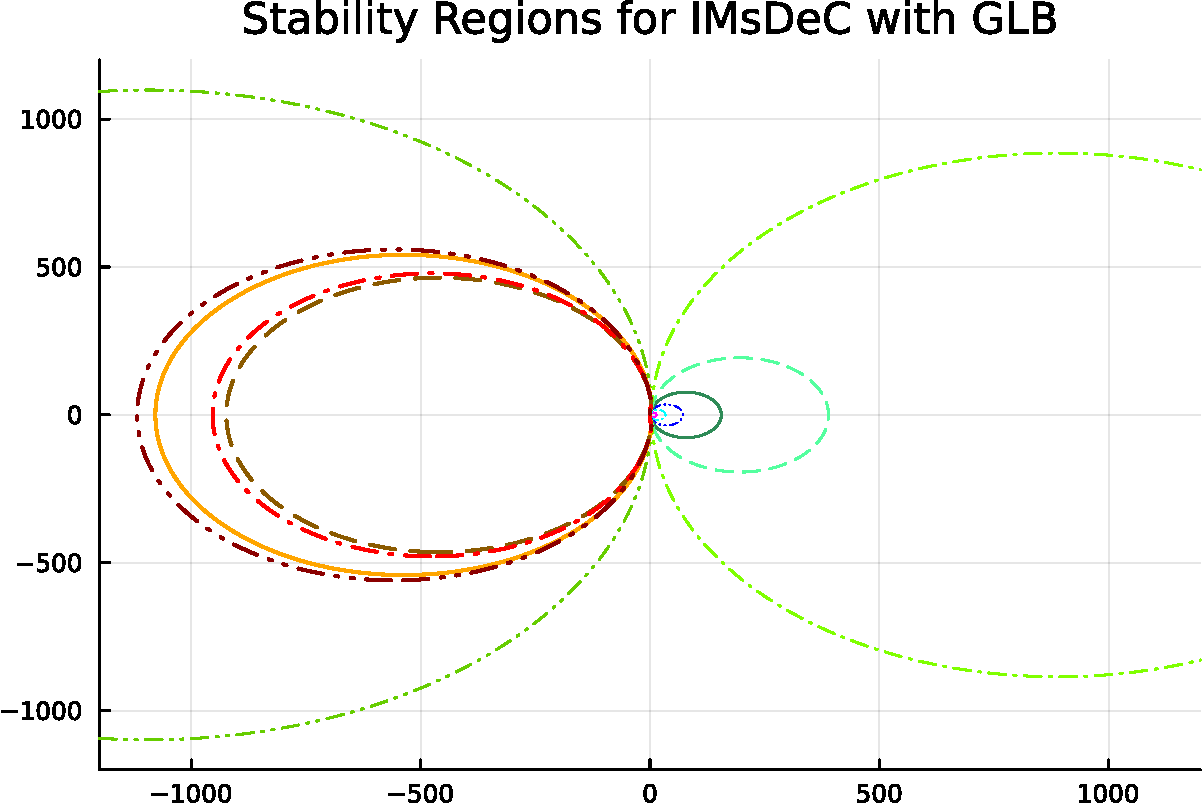
\includegraphics[width=\textwidth, trim={0 0 0 0}, clip]{pdf/odepics/IMsDeC_GLB_ord13-crop.pdf}\\
	ImsDeC GLB
	\end{minipage}
	\begin{minipage}[t]{0.32\textwidth}
		\centering
		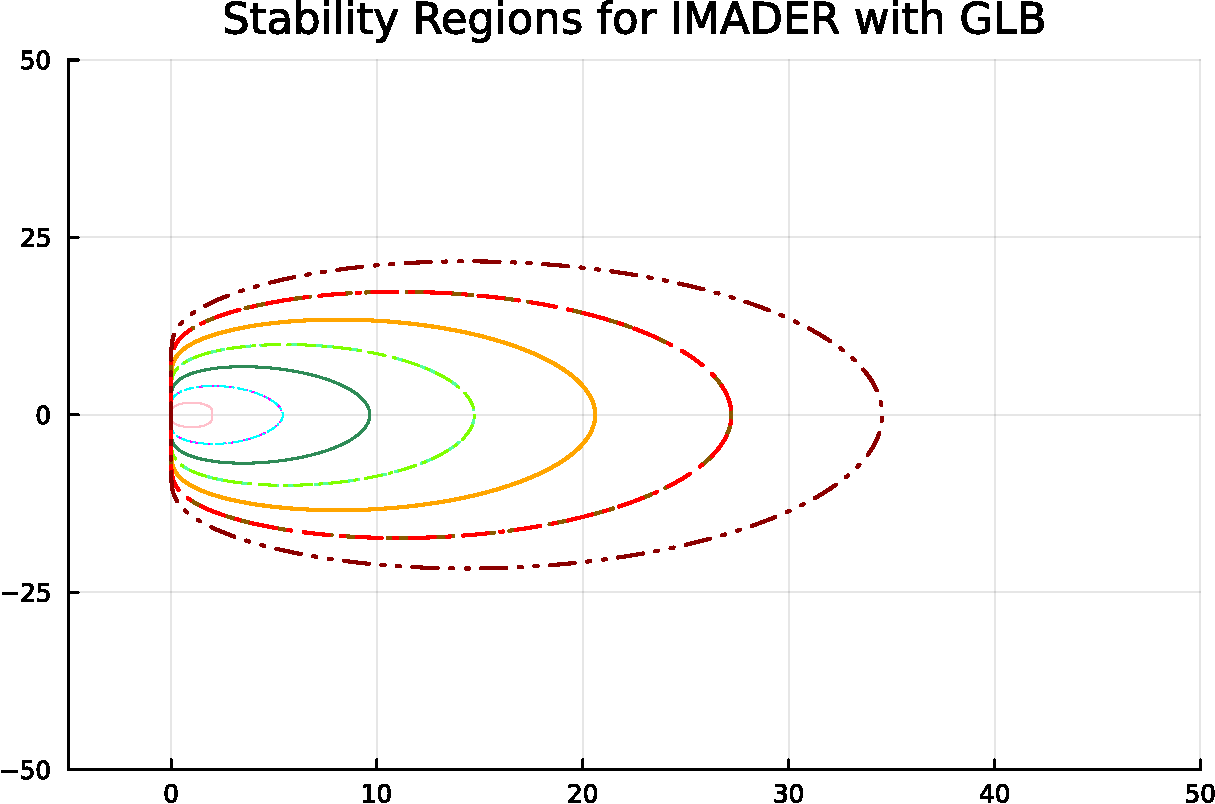
\includegraphics[width=\textwidth, trim={0 0 0 0}, clip]{pdf/odepics/IMADER_GLB_ord13-crop.pdf}\\
		ImADER GLB
	\end{minipage}
	\caption{Implicit DeC (left), sDeC (center) and ADER (right) with equispaced (top) and Gauss-Lobatto (bottom) nodes for orders 2 to 13}
	\label{fig: ODEIMDeCADER}
\end{figure}

\begin{figure}
	\centering
	\begin{minipage}[t]{0.33\textwidth}
		\centering
		\includegraphics[width=\textwidth, trim={0 0 0 0}, clip]{pdf/odepics/ImsDeC_eq_ord20-crop.pdf}\\
		ImsDeC eq
	\end{minipage}
	\begin{minipage}[t]{0.33\textwidth}
		\centering
		\includegraphics[width=\textwidth, trim={0 0 0 0}, clip]{pdf/odepics/ImsDeC_GLB_ord20-crop.pdf}\\
		ImsDeC GLB
	\end{minipage}
	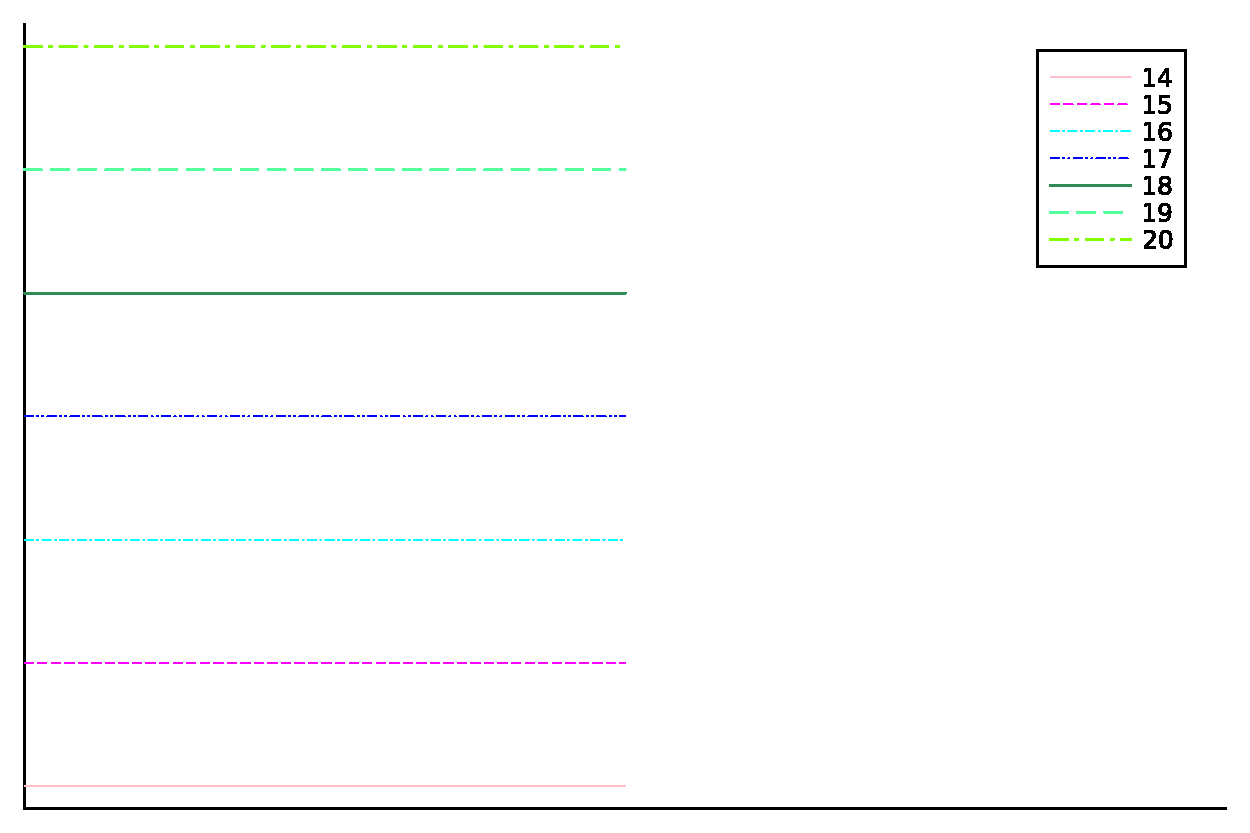
\includegraphics[width=0.1\textwidth, trim={491 230 30 23}, clip]{pdf/odepics/colors_a-d_new_14-20_no_order.pdf}
	\caption{Implicit sDeC for orders 14 to 20}
	\label{fig: exaImsDeC_high}
\end{figure}
The stability regions for the implicit sDeC (ImsDeC) are also shown in Figure~\ref{fig: ODEIMDeCADER} and, surprisingly, do not behave like the other methods. 
Up to a certain order (i.e. sDeC8 with Gauss-Lobatto and sDeC11 with equispaced nodes), the stability regions are unbounded and \textit{seem} A-stable, but for higher orders, we lose this property, obtaining large, but finite, stability regions. 
This behavior is not uniform and, at certain orders, the stability region will be unbounded again, as for example shown in Figure~\ref{fig: exaImsDeC_high} for very high order ImsDeC. 

%A legend for these plots can be found in figure~\ref{fig: legend_high_order}.
%\begin{figure}[!h]
%	\centering
%	\begin{minipage}[t]{0.18\textwidth}
%		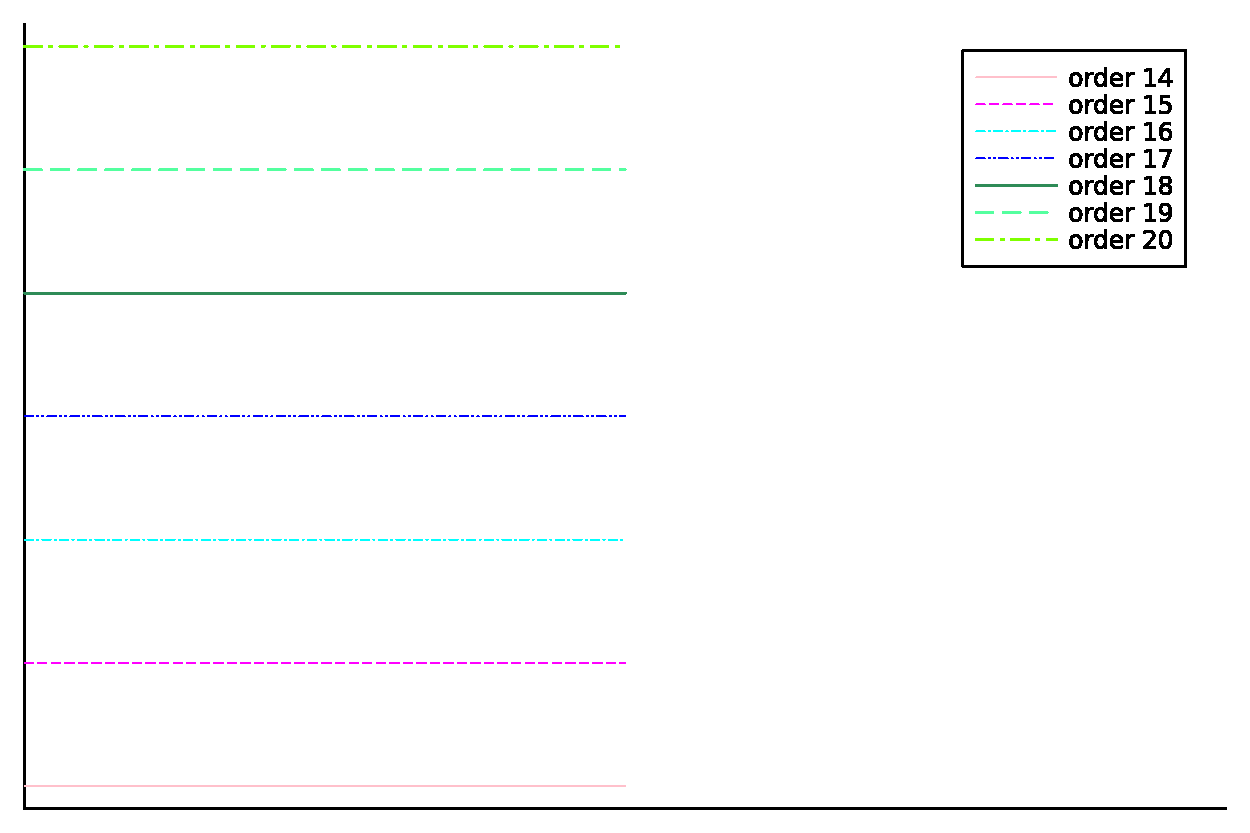
\includegraphics[width=\textwidth, trim={461 270 30 23}, clip]{pdf/odepics/colors_a-d_new_14-20.pdf}
%	\end{minipage}
%	\caption{Legend for the higher order Im sDeC methods.}
%	\label{fig: legend_high_order}
%\end{figure}

\begin{table}
	\centering
	\caption{Table with orders of the ImsDeC methods that have a bounded stability region on the negative half-plane}
	\label{tab:imsDeC_bounded}
	\begin{tabular}[h]{|c|c|}
		\hline
		ImsDeC nodes specification & orders of the method\\
		\hline
		Gauss-Lobatto & $9, 10, 11, 12, 13, 14, 15 $\\
		\hline	equispaced & $12, 13, 16, 17, 18, 19, 20 $\\
		\hline
	\end{tabular}
\end{table}
%Remark that the outlines of these stability regions can display inner or outer bounds as described before. Thereby, the shapes of these bounded stability regions mostly seem to be elliptic shaped. 
A detailed list of the bounded methods until order 20 is given in Table~\ref{tab:imsDeC_bounded}. 
%Why we use the term unbounded instead of A-stable will be discussed shortly afterwards.\\
For the sDeC, we can conclude that the choice of an implicit version does not guarantee an unbounded stability region. Nevertheless, even these implicit sDeC methods have larger stability regions than their explicit counterparts and therefore may be applicable to mildly stiff problems. 
We notice again that this odd loss of stability in the left half plane could not be found in the ImDeC and ImADER methods. We checked it numerically up to order 50.




\begin{figure}
	\centering
 	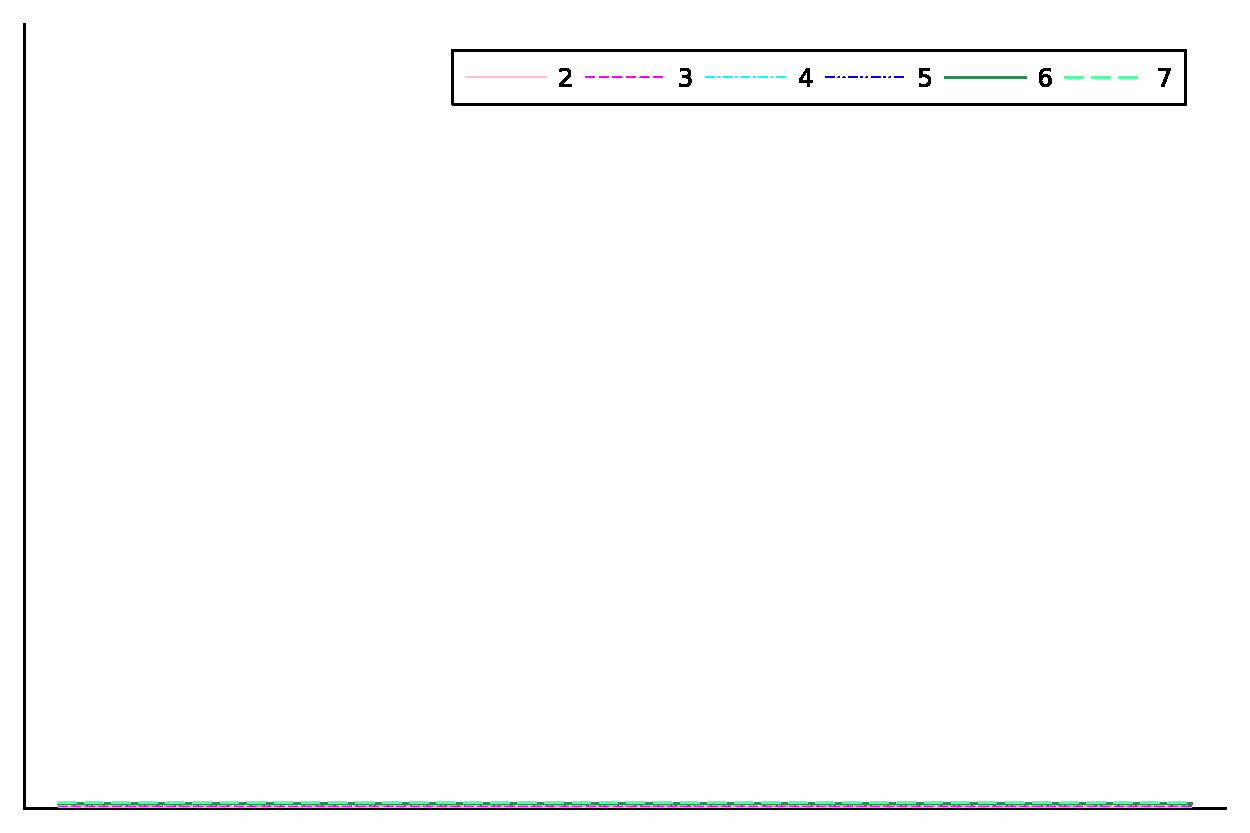
\includegraphics[width=0.465\textwidth,trim={215 340 33 22}, clip]{pdf/odepics/colors_a-d_new_horiz_2-7_no_order.pdf}\!\!
	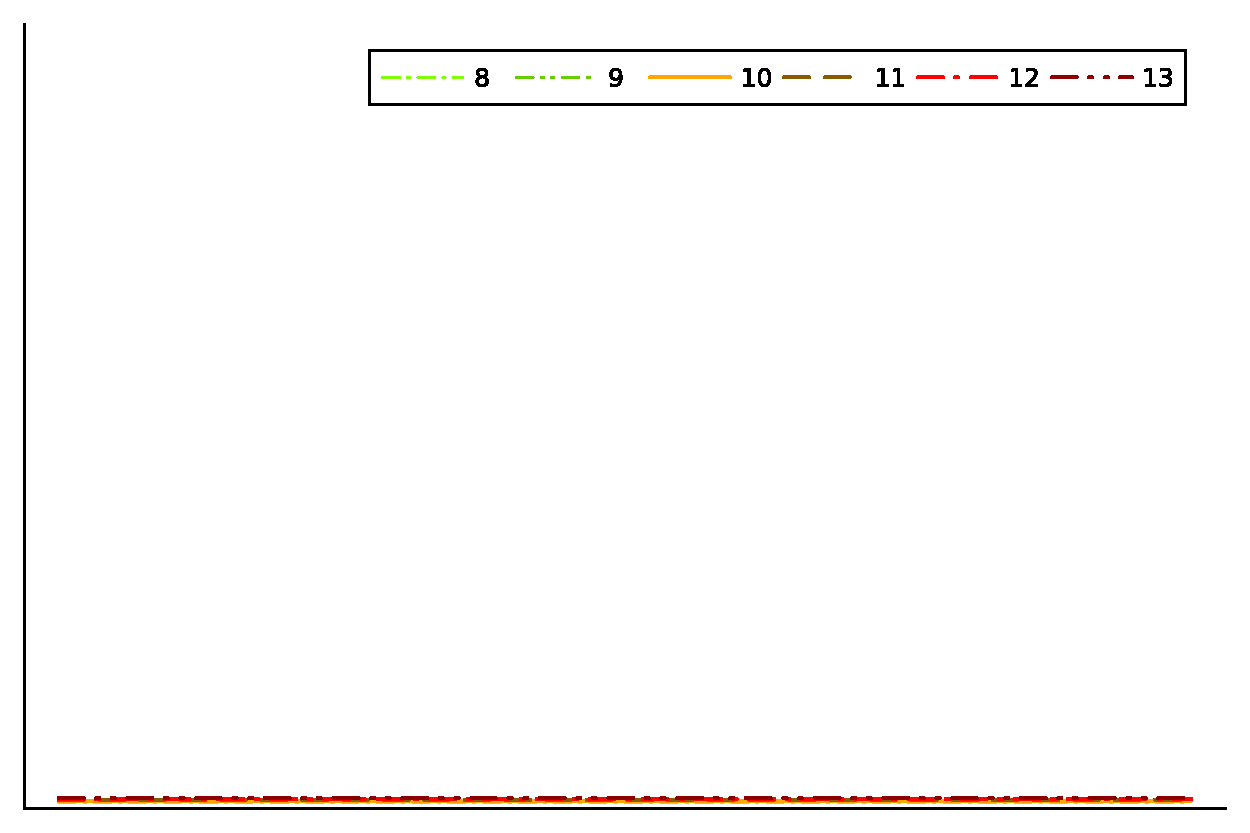
\includegraphics[width=0.515\textwidth,trim={179 340 30 22}, clip]{pdf/odepics/colors_a-d_new_horiz_8-13_no_order.pdf}\\

	\begin{minipage}[t]{0.325\textwidth}
		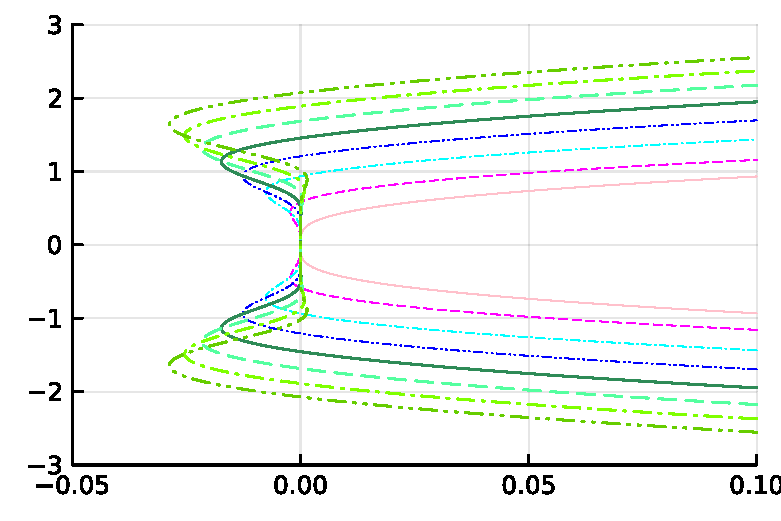
\includegraphics[width=\textwidth]{pdf/odepics/IMEXDeC_equispaced_zoom.pdf}
		\centering
		ImDeC eq from order 2 to 9
	\end{minipage}
	\begin{minipage}[t]{0.325\textwidth}
		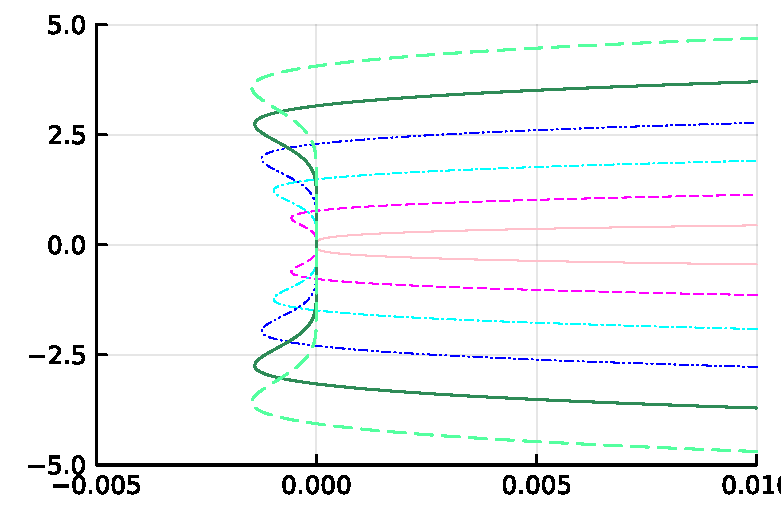
\includegraphics[width=\textwidth,trim={0 0 3 0}, clip]{pdf/odepics/IMEXDeC_subtimesteps_equispaced_zoom.pdf}
		\centering
		ImsDeC eq from order 2 to 7
	\end{minipage}
	\begin{minipage}[t]{0.325\textwidth}
		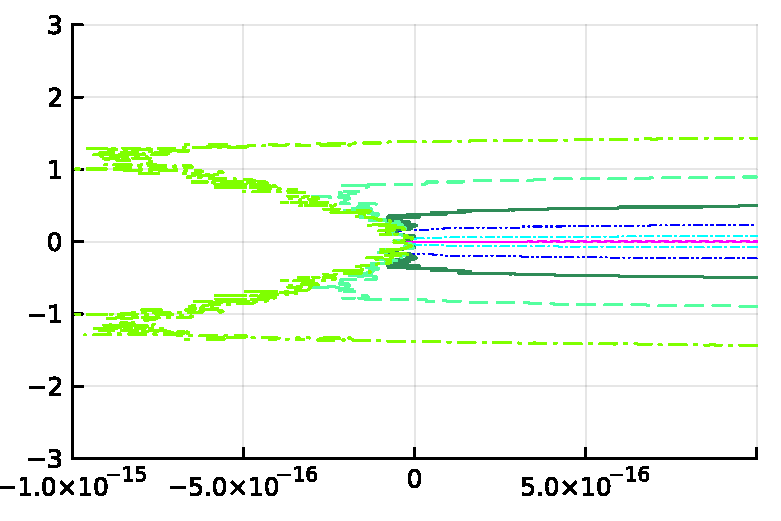
\includegraphics[width=\textwidth]{pdf/odepics/IMEXADER_equispaced_zoom.pdf}
		\centering
		ImADER eq from orders 3 to 8
	\end{minipage}\\[2mm]
	\begin{minipage}[t]{0.325\textwidth}
		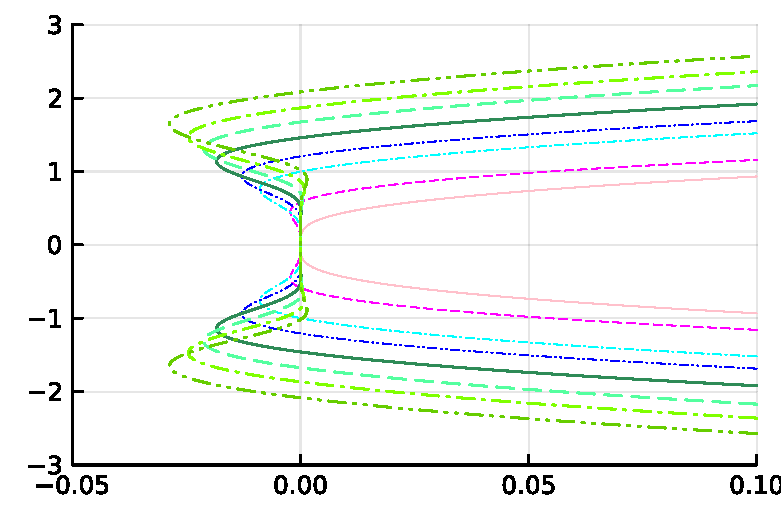
\includegraphics[width=\textwidth]{pdf/odepics/IMEXDeC_gaussLobatto_zoom.pdf}
		\centering
		ImDeC GLB from order 2 to 9
	\end{minipage}	
	\begin{minipage}[t]{0.325\textwidth}
		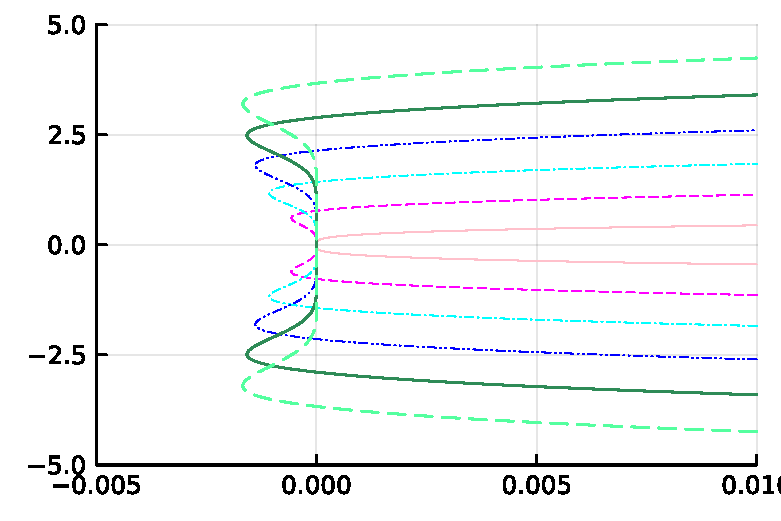
\includegraphics[width=\textwidth,trim={0 0 3 0}, clip]{pdf/odepics/IMEXDeC_subtimesteps_gaussLobatto_zoom.pdf}
		\centering
		ImsDeC GLB from orders 2 to 7
	\end{minipage}
	\begin{minipage}[t]{0.325\textwidth}
		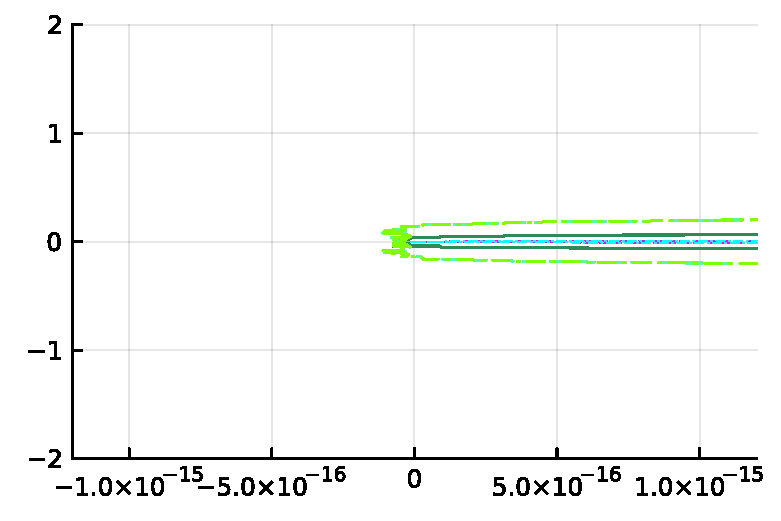
\includegraphics[width=\textwidth]{pdf/odepics/IMEXADER_gaussLobatto_zoom.pdf}
		\centering
		ImADER GLB from orders 3 to 8
	\end{minipage}
	\caption{Zoomed stability region of implicit schemes (watch out at the different scales).}
	\label{fig: ODE_minor_instabilitys}
\end{figure}

Taking a closer look at the implicit methods, we additionally detect some minor instability regions on the negative half-plane, see Figure~\ref{fig: ODE_minor_instabilitys}.
It turns out that these instabilities appear for all ImDeC and ImsDeC methods of orders larger than 2 and both types of nodes. We display the sDeC only with GLB nodes, as the equispaced nodes version is very similar to that.
For a very small scale, the same can be seen for the ImADER methods with equispaced nodes of orders at least larger than 4, displayed on the top right of Figure~\ref{fig: ODE_minor_instabilitys}. 
Notice that the sizes of the unstable regions are close to machine precision, which results in non-smooth boundaries and it is unclear if the ImADER with equispaced nodes are not A-stable or the visualization of the unstable area is given by machine precision errors.

As proved in \cite{petri2024analysis}, also numerically we observe that the ImADER methods with Gauss-Lobatto nodes are A-stable for all orders. Here, the noise in the stability region (bottom right of Figure~\ref{fig: ODE_minor_instabilitys}) is really of the size of machine precision.

%Hence, we classify the implicit methods as A-stable, \textit{almost A-stable}, when the stability region is unbounded and it \textit{almost} includes the whole left half--plane, or with bounded stability region.
%Remark that for \textit{almost A-stable} methods these minor instabilities do not influence the behavior of the scheme on many stiff problems. Nevertheless, when the eigenvalues $\lambda$ of the system are (almost) purely imaginary, they might encounter instabilities for some discretizations.
%, so that for certain step-sizes $\Delta t$ it is possible to get a $z=\lambda \Delta t$ located in the unstable region.


Summarizing, we can categorize our methods in 3 different classes: 
\begin{itemize}
	\item The A-stable schemes: all ImADER GLB and all second order implicit methods;
	\item The \textit{almost A-stable} schemes, when the stability region is unbounded and it \textit{almost} includes the whole left half--plane: high order ImDeC, some ImsDeC and ImADER equispaced;
	\item The bounded stability schemes: some ImsDeC.
\end{itemize}

Remark that for \textit{almost A-stable} methods these minor instabilities do not influence the behavior of the scheme on many stiff problems. Nevertheless, when the eigenvalues $\lambda$ of the system are (almost) purely imaginary (typical for high order advection operators), they might encounter instabilities for some discretizations.

\subsection{IMEX schemes}
To study the stability of IMEX schemes, we will use the RK stability function 
%We will now evaluate our constructed IMEX methods, by using their Butcher tableaux 
%\begin{equation}\label{eq:ImExButcherTableu}
%\begin{array}{c|c}
%c & A\\\hline
%& b^T
%\end{array}, \qquad
%\begin{array}{c|c}
%c & \hat{A}\\\hline
%& \hat{b^T}
%\end{array}.
%\end{equation}
%to receive their stability functions
\begin{equation}\label{eq:ImExStabilityFunction}
R(z_I, z_E)=1+\left(z_I\vec{b}^T+z_E\vec{\hat{b}}^T\right)\vec{u}=1+\left(z_I\vec{b}^T+z_E\vec{\hat{b}}^T\right)\left(\mat{Id}-z_I\mat{A}-z_E\mat{\hat{A}}\right)^{-1} \vec{1}
\end{equation}
that uses the matrices defined by the Butcher tableau of an IMEX RK.
Remark that the standard approach of A-stability cannot be used anymore.
Indeed, the region of absolute stability $$S=\left\{(z_I,z_E)\in \mathbb{C}^2 \ : \ \lvert{R(z_I,z_E)}\rvert\le1\right\}$$ lays in a larger space, with respect to classical RK schemes, therefore, its study, computation and visualization are challenging.
%Like in the classic case, we do not need (and do not want) the whole region $\mathbb{C}^2$ for satisfying results besides the issue of problematic visualization. Here arises the question which subsets of stability we want to consider. \\
Hence, we need to rely on some simplifications.
In \cite{minion2003dec}, Minion simplifies the Dahlquist equation by imposing
\begin{equation*}
\lambda_I \in \mathbb{R}, \quad \lambda_E =i\lambda_E', \ \lambda_E' \in \mathbb{R}.
\end{equation*} 
This procedure neglects respectively the imaginary or real part of the coefficients in the Dahlquist equation to display a two-dimensional region. This idea is lead by classical PDE discrete operators, where typically the diffusion is symmetric negative definite, while the advection is mainly with imaginary eigenvalues. 
A second approach where for each $\lambda_E$ the A-stability is required for the implicit part of the scheme was originally studied in \cite{zhong1996additive,caflisch1997uniformly} and formalized in \cite{liotta2000central}. Another approach studies, instead, the stability for each $\lambda_I$ requiring at least the stability region of the explicit Euler method to the explicit part \cite{Hundsdorfer}.
We collect these definitions of stability region in the following.
\begin{definition}[Stability regions]
	Consider the modified test equation with stability function \eqref{eq:ImExStabilityFunction}. Then, we define multiple approaches for IMEX stability regions by
	\begin{itemize}
		\item $S:=\left\{(z_I,z_E)\in \mathbb{C}^2 \ :\ \lvert{R(z_I,z_E)}\rvert\le1\right\}$ (Region of absolute stability),
	\item  $\mathcal{D}_M:= \left\{(z_I,z_E)\in \mathbb{R}^2 \ :\ \lvert{R(z_I,iz_E)}\rvert\le1\right\}$  (Minion's stability region) \cite{minion2003dec}, 
	\item  $\mathcal{D}_0:=\left\{z_E \in \mathbb{C}\ :\ \lvert{R(z_I,z_E)}\rvert \le 1 \textrm{ for any } z_I \in \mathbb{C}^- \right\}$ \cite{liotta2000central},
	\item $\mathcal{D}_1:=\left\{z_I \in \mathbb{C}\ :\ \lvert{R(z_I,z_E)}\rvert \le 1 \textrm{ for any } z_E \in \mathcal{S}_0 \right\}$ \cite{Hundsdorfer},
	\end{itemize}
	where $\mathcal{S}_0=\left\{z_E \in \mathbb{C}\ :\ \lvert 1+z_E\rvert \le 1 \right\}$ is the stability region of the explicit Euler method. 
\end{definition}
%Remark that $\mathbb{C}^-$ is the smallest stability region to fulfill the A-stability. 
%Hundsdorfer's definitions \cite{Hundsdorfer} $\mathcal{D}_0$ and $\mathcal{D}_1$ give statements about the explicit or implicit part of the equation, respectively assuming that the other part fulfills these known stability properties.
$\mathcal D_0$ is a very strict condition of IMEX stability, in particular for the considered high order schemes. 
%We will refer to $\mathcal{D}_M$ as Minion's stability approach and to $\mathcal{D}_0$ /\mathcal{D}_1$ as Hundsdorfer's stability approach.
Theoretically, the terms A-stability and A($\alpha$)-stability may be applied for all 3 of these subsets of $\mathbb{C}$ analogously to the classical cases, so we will make use of this terminology too. 

\subsubsection*{$\mathcal{D}_M$ stability region}
\begin{figure}
	\centering
	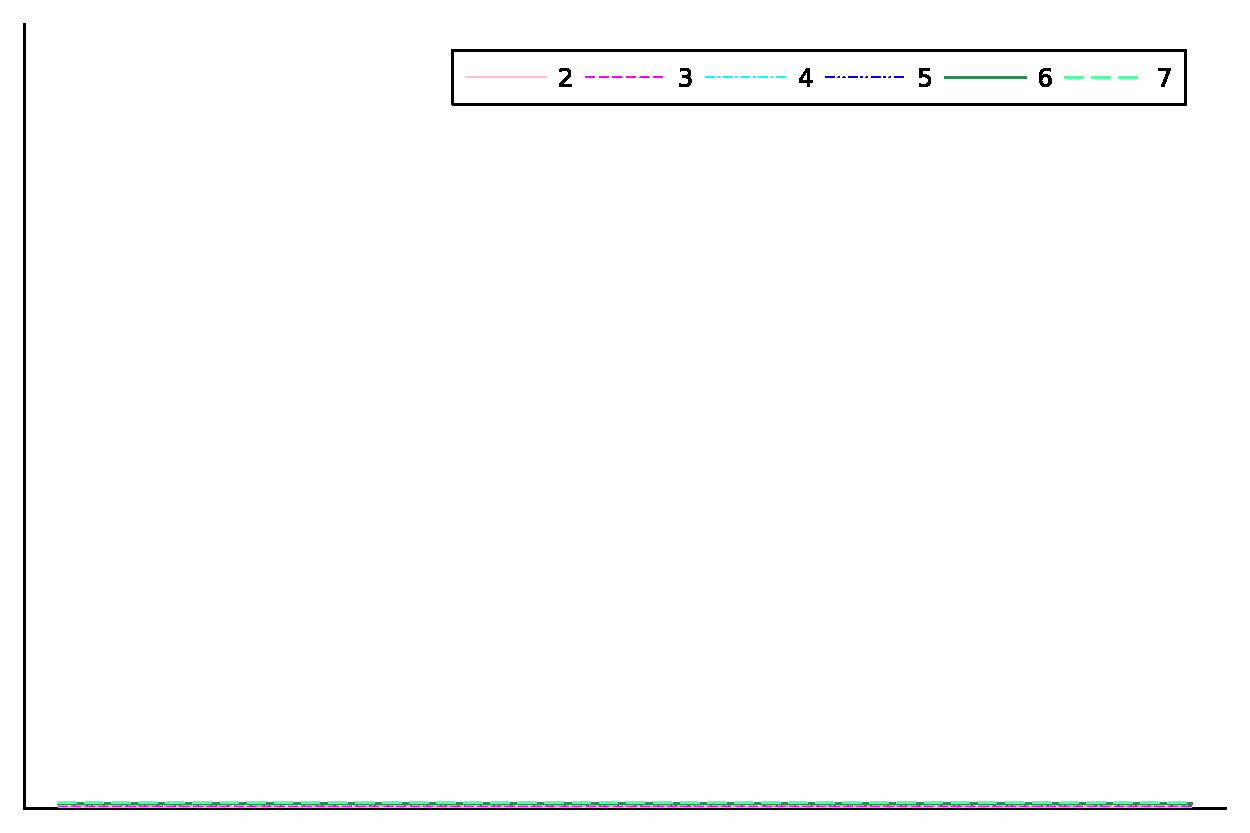
\includegraphics[width=0.465\textwidth,trim={215 340 32 22}, clip]{pdf/odepics/colors_a-d_new_horiz_2-7_no_order.pdf}\!\!
	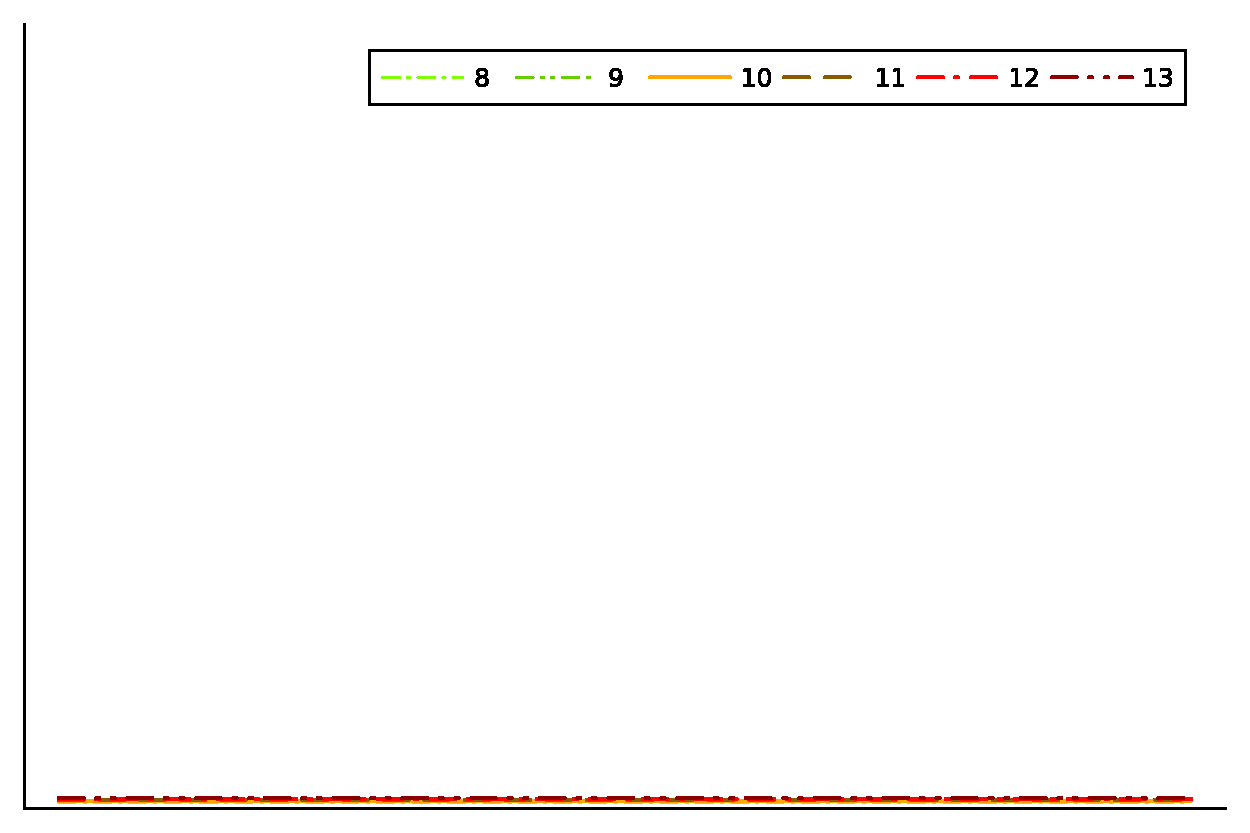
\includegraphics[width=0.515\textwidth,trim={179 340 30 22}, clip]{pdf/odepics/colors_a-d_new_horiz_8-13_no_order.pdf}\\
	\begin{minipage}[t]{0.32\textwidth}
		\centering
		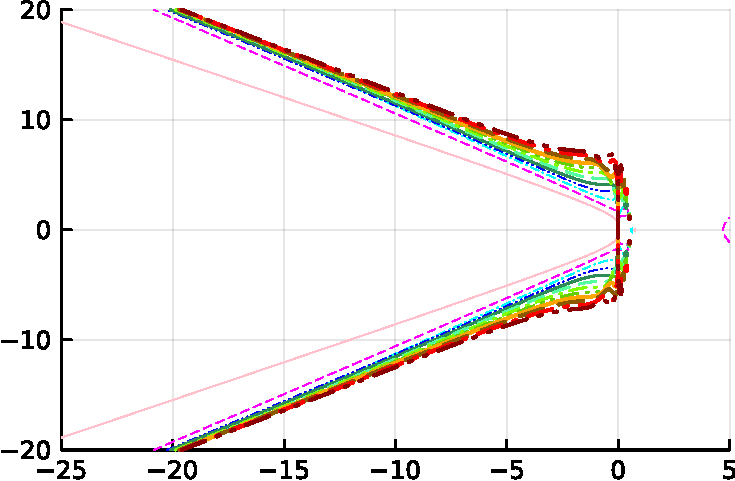
\includegraphics[width=\textwidth, trim={0 0 0 0}, clip]{pdf/odepics/Minion_IMEXDeC_eq_ord13-crop.pdf}
		IMEXDeC eq orders 2 to 13
	\end{minipage}	
	\begin{minipage}[t]{0.32\textwidth}
		\centering
		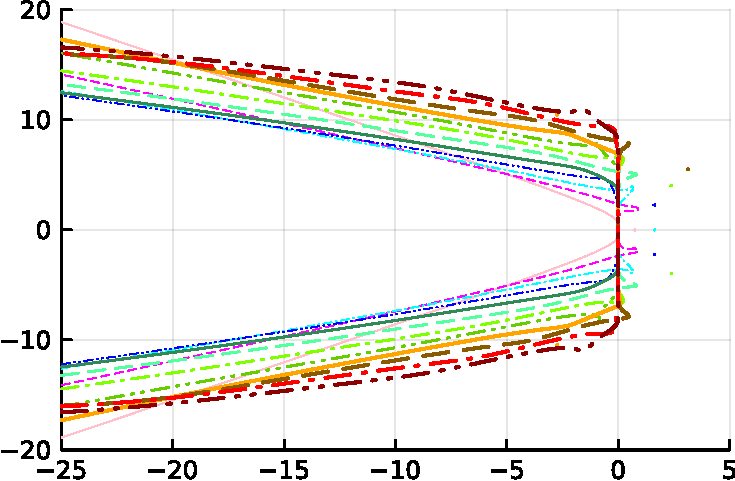
\includegraphics[width=\textwidth, trim={0 0 0 0}, clip]{pdf/odepics/Minion_IMEXsDeC_eq_ord13-crop.pdf}
		IMEXsDeC eq orders 2 to 13
	\end{minipage}
	\begin{minipage}[t]{0.32\textwidth}
		\centering
		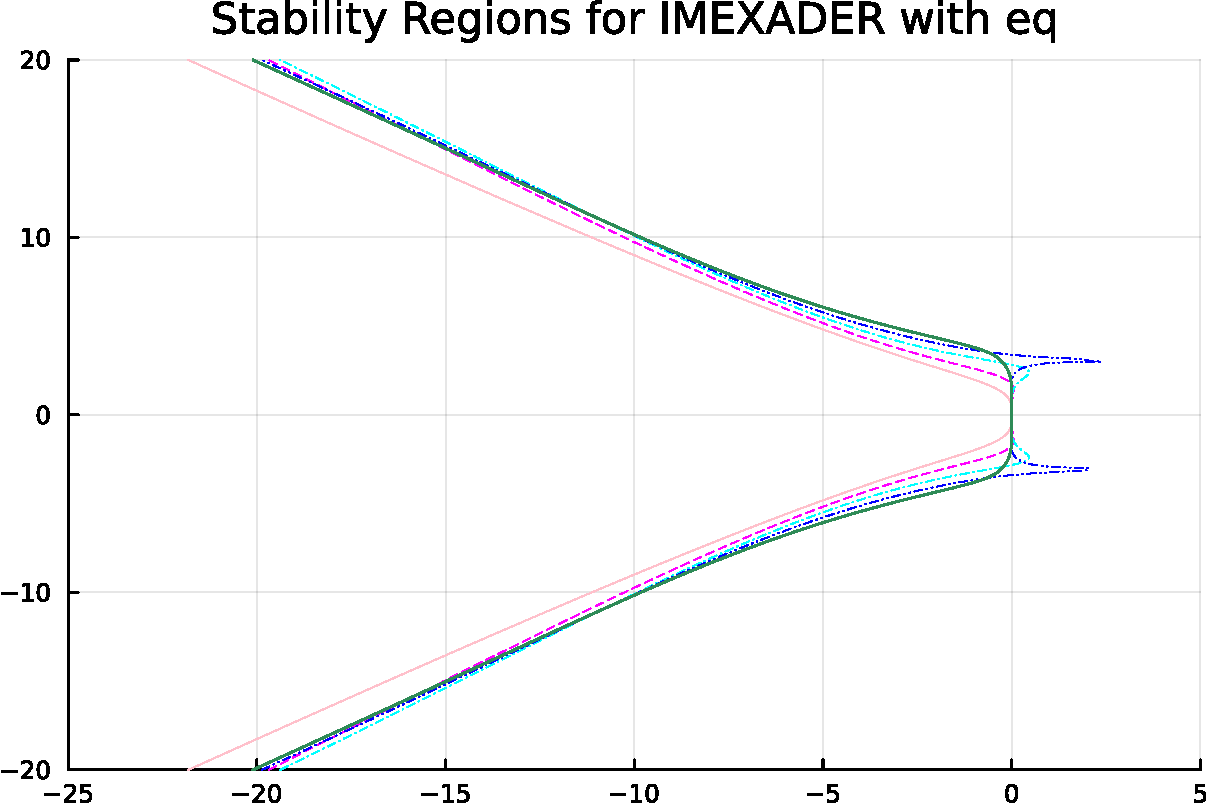
\includegraphics[width=\textwidth, trim={0 0 0 0}, clip]{pdf/odepics/Minion_IMEXADER_eq_ord6-crop.pdf}
		IMEXADER eq orders 2 to 6
	\end{minipage}\\[2mm]
	\begin{minipage}[t]{0.32\textwidth}
		\centering
		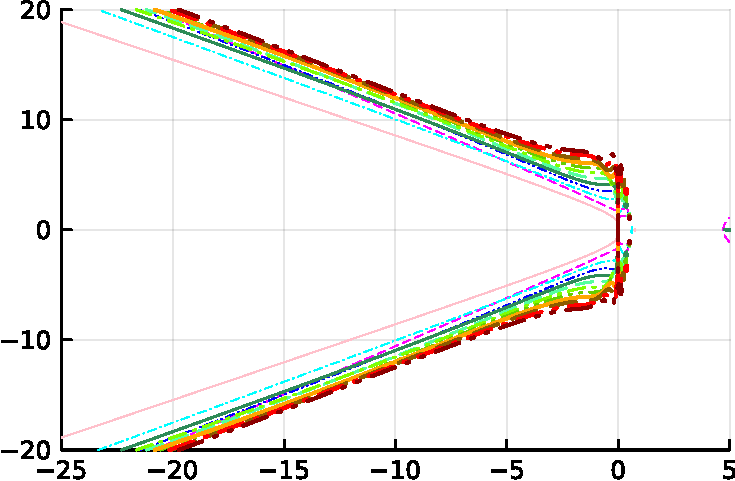
\includegraphics[width=\textwidth, trim={0 0 0 0}, clip]{pdf/odepics/Minion_IMEXDeC_GLB_ord13-crop.pdf}
		IMEXDeC GLB orders 2 to 13
	\end{minipage}
	\begin{minipage}[t]{0.32\textwidth}
		\centering
		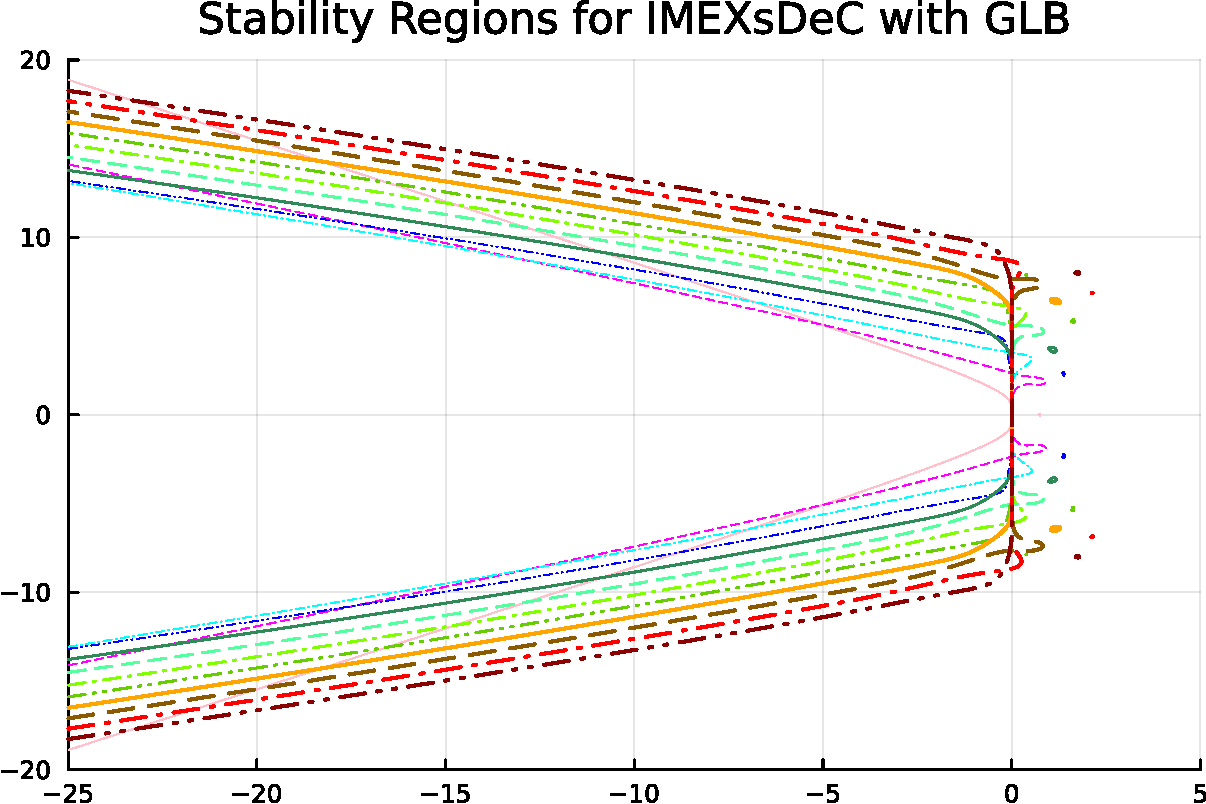
\includegraphics[width=\textwidth, trim={0 0 0 0}, clip]{pdf/odepics/Minion_IMEXsDeC_GLB_ord13-crop.pdf}
		IMEXsDeC GLB orders 2 to 13
	\end{minipage}
	\begin{minipage}[t]{0.32\textwidth}
		\centering
		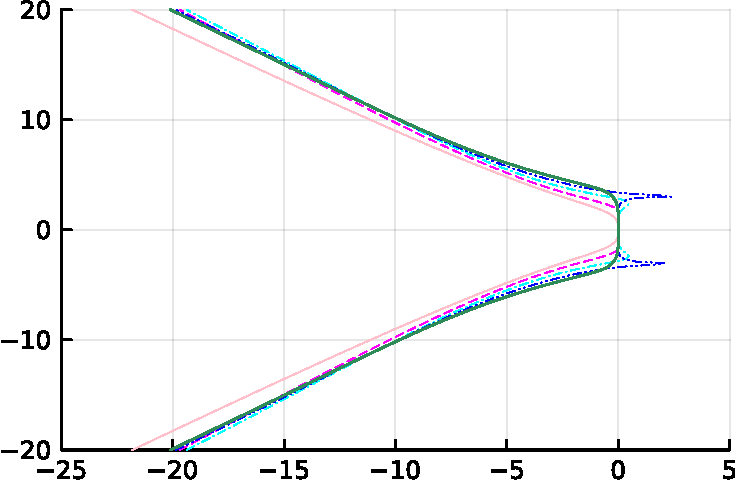
\includegraphics[width=\textwidth, trim={0 0 0 0}, clip]{pdf/odepics/Minion_IMEXADER_GLB_ord6-crop.pdf}
		IMEXADER GLB orders 2 to 6
	\end{minipage}
	\caption{Minion's stability region for IMEX DeC (left), sDeC (center) and ADER (right) with equispaced (top) and GLB (bottom) nodes}
	\label{fig: ODEIMEX}
\end{figure}
We recall that the plots of the stability regions have very different meaning according to the chosen approach. 
%Considering the previously developed IMEX methods, we want to recall that the view on the regions of stability changes, depending on the approach we choose. Firstly, we want to consider stability like in \cite{minion2003dec}. 
%It is possible to write the method used there into the IMEX sDeC method, so we expect the same results as him in \cite[fig. 4.1]{minion2003dec}. 
Starting from Minion's approach \cite{minion2003dec}, we evaluate the IMEX stability function \eqref{eq:ImExStabilityFunction} numerically to calculate the respective stability regions. 

For the IMEX DeC, we can observe in Figure~\ref{fig: ODEIMEX} (left) that the choice of nodes change the regions on some details but the qualitative behavior is the same. We can also conclude on an $A(\alpha)-$stability for approximately $\alpha=35^\circ$.

Going on to the IMEX ADER, we can see in Figure~\ref{fig: ODEIMEX} (right) a similar behavior, even if the stability regions differ in small details, we observe $A(\alpha)-$stability for at least $\alpha=35^\circ$.

Finally, for the IMEX sDeC method in Figure~\ref{fig: ODEIMEX} (center) we see a slightly different behavior, still resulting in an $A(\alpha)-$stability, but for significantly smaller angles, approximately $\alpha=18^\circ$. 
%Remark that this is significantly lower than for both the IMEX ADER and IMEX DeC. 
Nevertheless, the result on the bottom center in Figure~\ref{fig: ODEIMEX} with GLB nodes coincides with the one in \cite{minion2003dec}, as expected. 
%So we can conclude that the IMEX variations for all of these methods also have a somehow similar $A(\alpha)-$stability for some $\alpha>10^\circ$, at least for this view on the stability for IMEX methods.\\
It is also noticeable that the IMEX sDeC stability region of order 2 is $A(\alpha)$-stable with larger $\alpha$ as it coincides with the IMEX DeC2.

With the $\mathcal{D}_M$ approach, we do not observe strong variations between equispaced and Gauss--Lobatto points.


\subsubsection*{$\mathcal{D}_0$ stability region}

Now, we want to evaluate $\mathcal{D}_0$ stability for our IMEX methods. 
We want to emphasize that the requirements here are stricter than in Minion's approach. 
Indeed, for $\mathcal{D}_0$ we require the method to be at least fully A-stable for the implicit part and we look at the stability of the explicit part.
The IMEX DeC and IMEX sDeC have $\mathcal{D}_0=\emptyset$ and this is probably related to the fact that their implicit counterpart is not A-stable.
For the IMEX ADER, only few orders have non-empty $\mathcal{D}_0$ stability region. In Figure~\ref{fig: HundsdorferD0_IMEXADER}, we show the few stability regions, which eventually vanish when increasing the order of accuracy.
\begin{figure}
	\centering
	\begin{minipage}[t]{0.4\textwidth}
		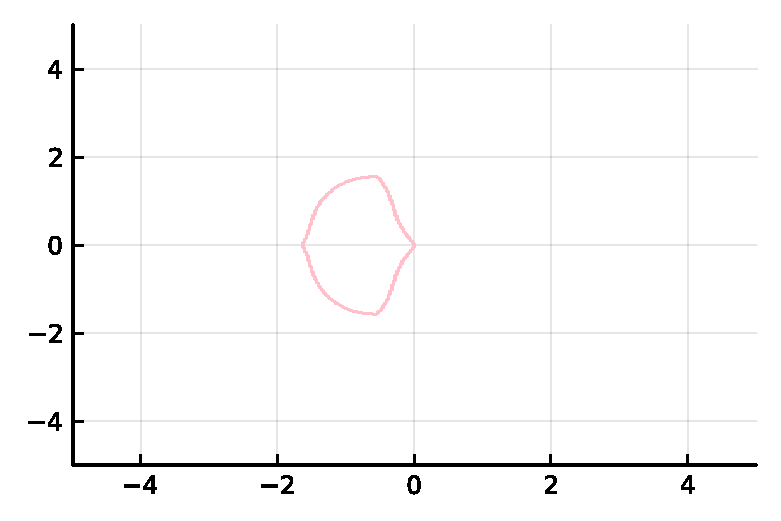
\includegraphics[width=\textwidth]{pdf/odepics/ImExD0_IMEXADER_equispaced.pdf}
		\centerline{Order 2 with equispaced nodes}
	\end{minipage}\,\,
	\begin{minipage}[t]{0.4\textwidth}
		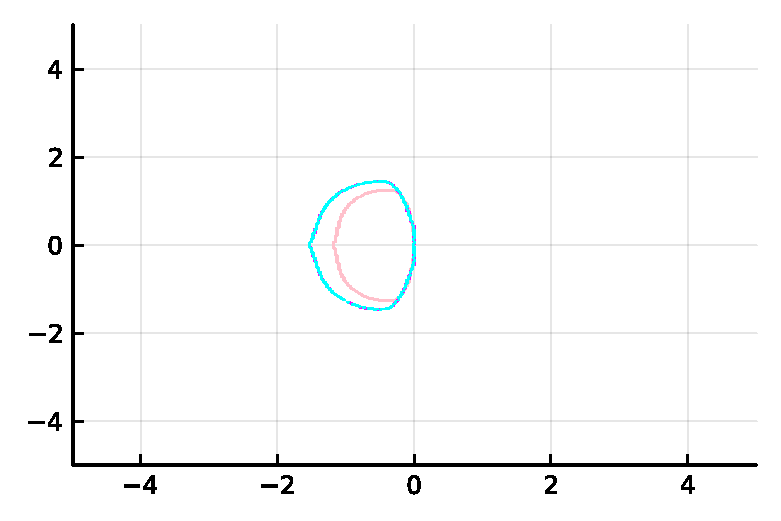
\includegraphics[width=\textwidth]{pdf/odepics/ImExD0_IMEXADER_gaussLobatto.pdf}
		\centerline{Orders 2 to 4 with Gauss-Lobatto nodes}
	\end{minipage}
	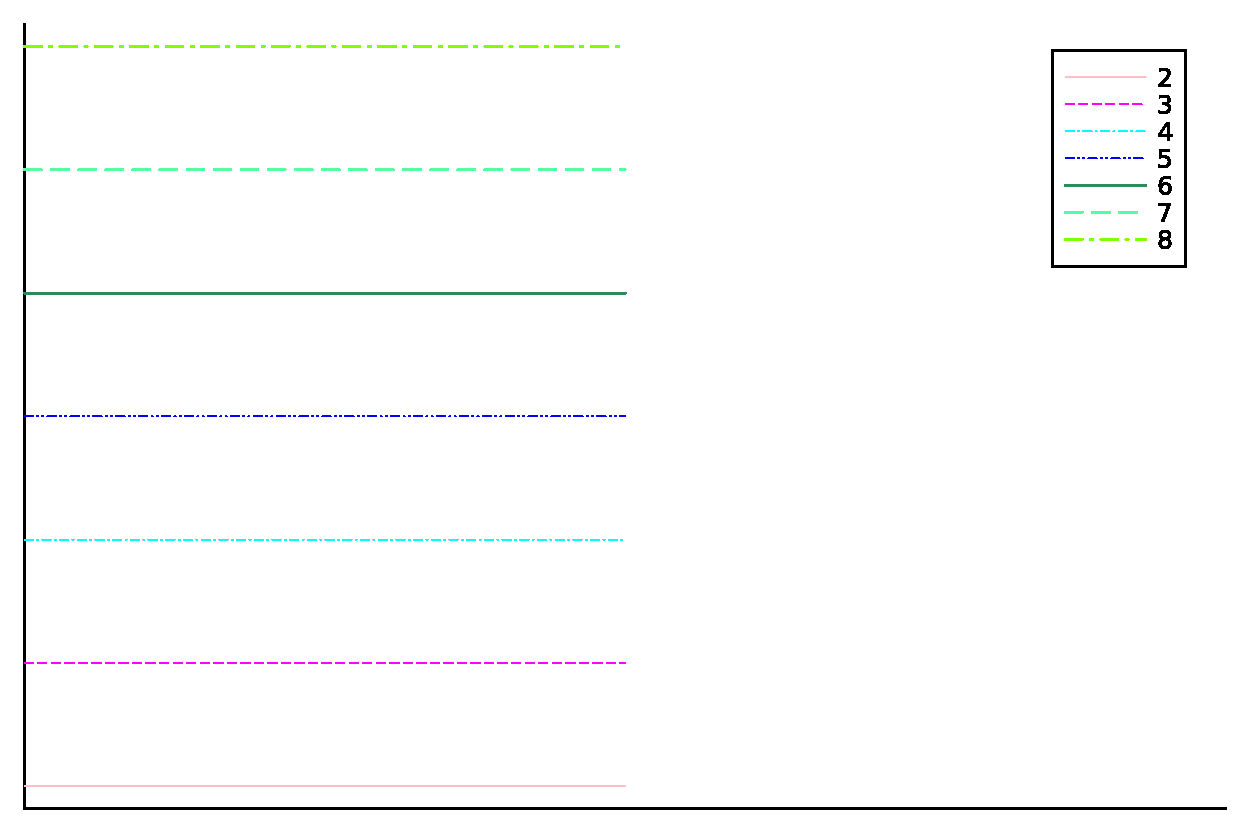
\includegraphics[width=0.12\textwidth, trim={491 230 30 23}, clip]{pdf/odepics/colors_a-d_new_2-8_no_order.pdf}
	\caption{$\mathcal{D}_0$ Stability regions for IMEX ADER. The smaller stability region displays order 2, while the larger one displays order 3 and 4 (right)}
\label{fig: HundsdorferD0_IMEXADER}
\end{figure}

\subsubsection*{$\mathcal{D}_1$ stability region}
We plot the $\mathcal{D}_1$ stability regions for DeC and sDeC methods in Figures~\ref{fig: HundsdorferD1_IMEX}, where we require the explicit part to cover the stability region of the explicit Euler method and we look at the stability of the implicit part.
Contrary to the $\mathcal{D}_0$ cases, we observe non-empty, limited regions of stability for every order for the IMEX DeC methods. Moreover, there is no regularity in their shape and their size grow significantly as the order of accuracy increases.
Notice that the plots do not show the full stability regions of higher orders, for example for orders 6, 7, and 8 with equispaced nodes, but they are anyway bounded regions. \\
For the IMEX sDeC, see Figure~\ref{fig: HundsdorferD1_IMEX} (center), we observe some remarkable differences. In the case of equispaced nodes, even orders just show the small bounded stability regions in the negative half-plane nearby the origin, odd orders smaller than 6 show large stability regions, while they are unstable starting from order 7. 
Also in the GLB case, we do not observe much regularity. 
We notice that the largest stability region is obtained for order 5, while, for higher orders, the stability region almost fit in the plot.
\begin{figure}
	\centering
	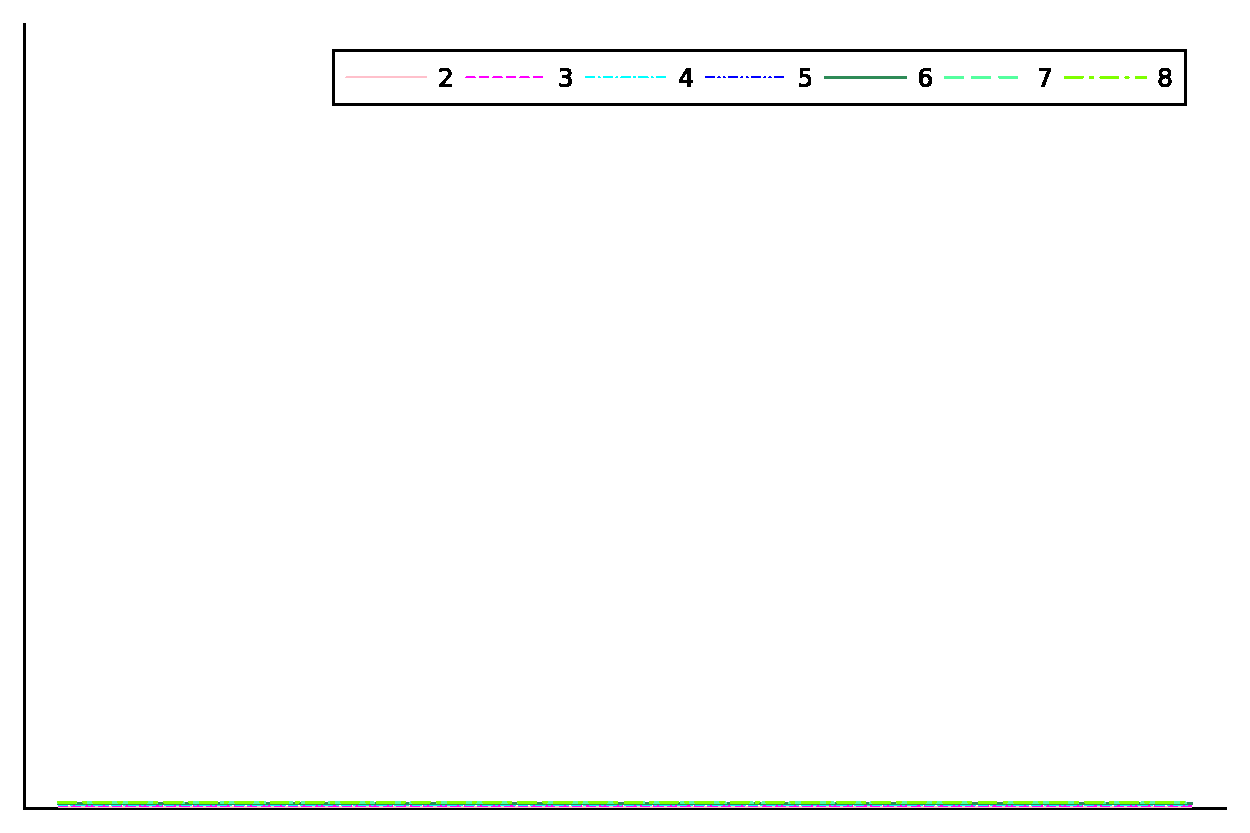
\includegraphics[width=0.515\textwidth,trim={158 340 30 22}, clip]{pdf/odepics/colors_a-d_new_horiz_2-8_no_order.pdf}\\
	\begin{minipage}[t]{0.32\textwidth}
		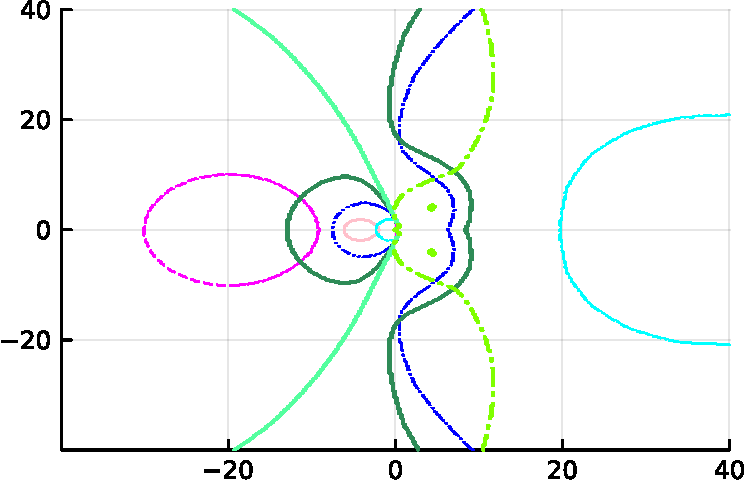
\includegraphics[width=\textwidth]{pdf/odepics/ImExD1_IMEXDeC_equispaced_range=40-crop.pdf}
		\centerline{IMEX DeC eq}
	\end{minipage}
	\begin{minipage}[t]{0.32\textwidth}
	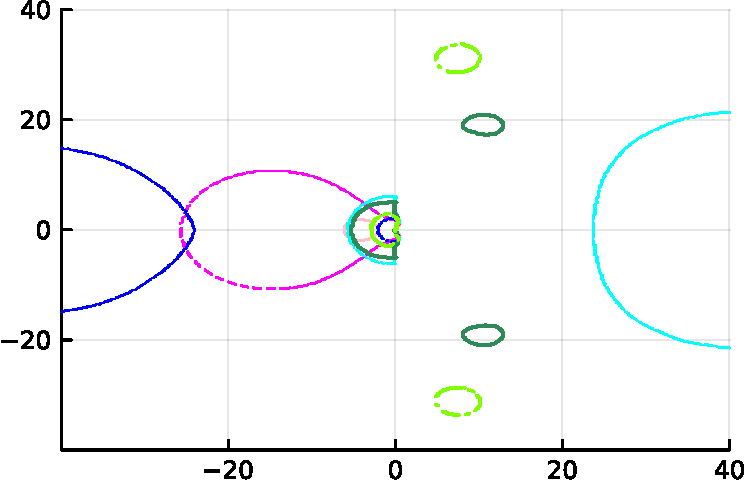
\includegraphics[width=\textwidth]{pdf/odepics/ImExD1_IMEXDeC_subtimesteps_equispaced_range=40-crop.pdf}
	\centerline{IMEX sDeC eq}
	\end{minipage}
	\begin{minipage}[t]{0.32\textwidth}
	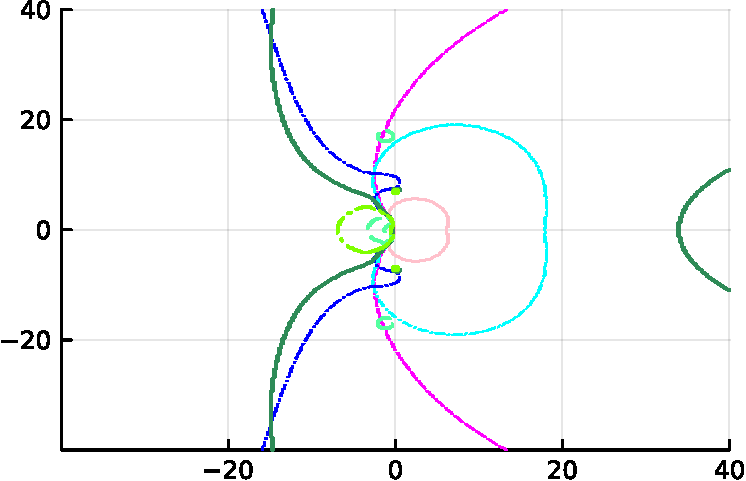
\includegraphics[width=\textwidth]{pdf/odepics/ImExD1_IMEXADER_equispaced_range=40-crop.pdf}
	\centerline{IMEX ADER eq}
	\end{minipage}\\
	\begin{minipage}[t]{0.32\textwidth}
	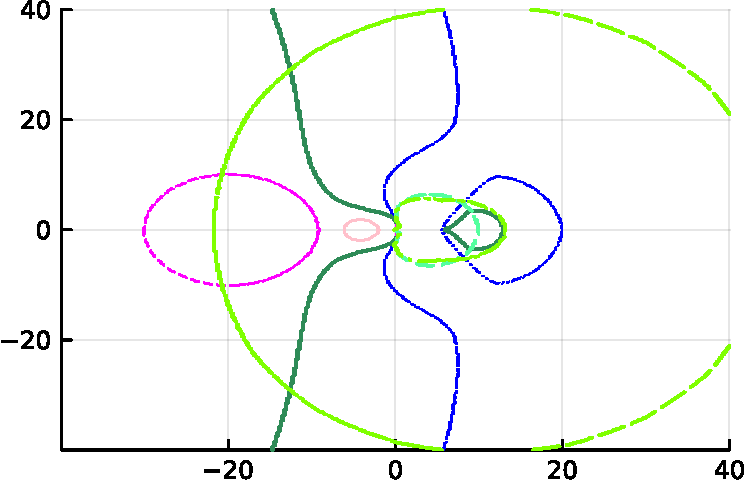
\includegraphics[width=\textwidth]{pdf/odepics/ImExD1_IMEXDeC_gaussLobatto_range=40-crop.pdf}
	\centerline{IMEX DeC GLB}
	\end{minipage}
	\begin{minipage}[t]{0.32\textwidth}
	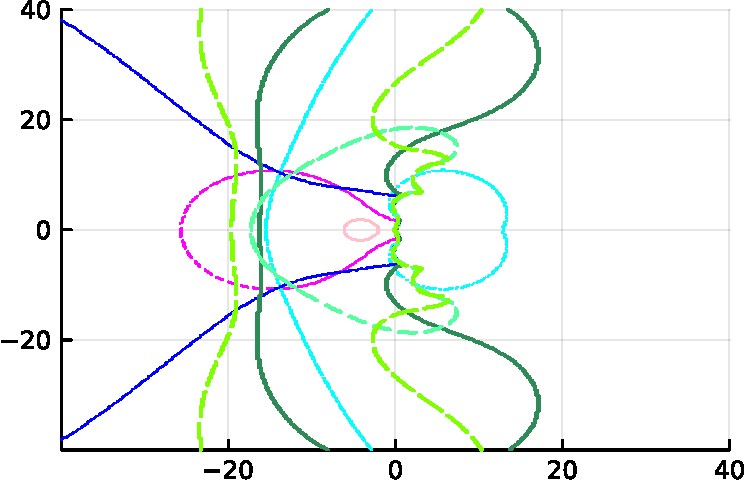
\includegraphics[width=\textwidth]{pdf/odepics/ImExD1_IMEXDeC_subtimesteps_gaussLobatto_range=40-crop.pdf}
	\centerline{IMEX sDeC GLB}
	\end{minipage}
	\begin{minipage}[t]{0.32\textwidth}
	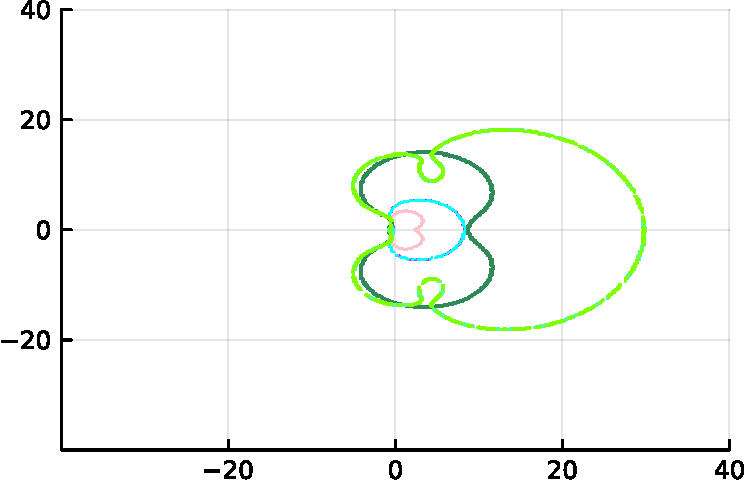
\includegraphics[width=\textwidth]{pdf/odepics/ImExD1_IMEXADER_gaussLobatto_range=40-crop.pdf}
	\centerline{IMEX ADER GLB}
	\end{minipage}
%	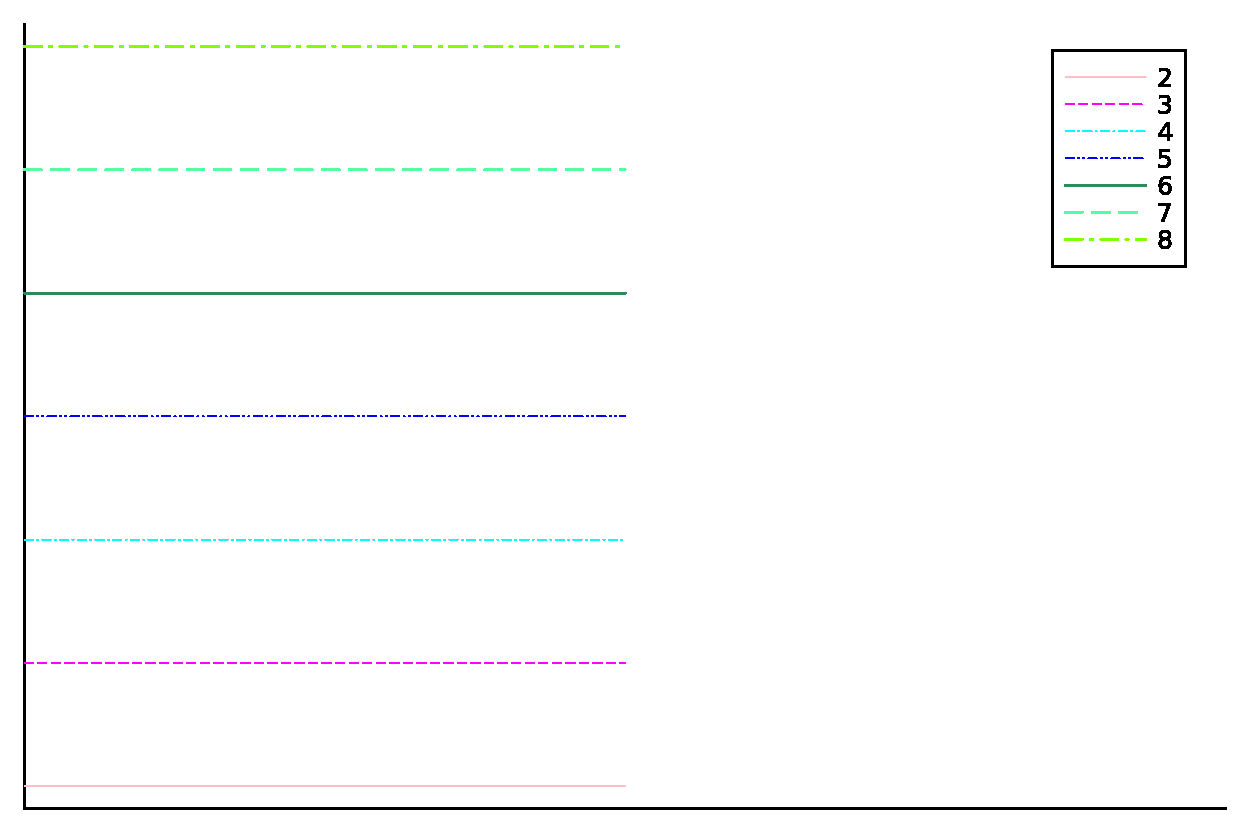
\includegraphics[width=0.08\textwidth, trim={491 180 30 23}, clip]{pdf/odepics/colors_a-d_new_2-8_no_order.pdf}
	\caption{$\mathcal{D}_1$ Stability Region for IMEX DeC (left), sDeC (center) and ADER (right) with equispaced (top) and GLB (bottom) nodes: orders 2 to 8}
\label{fig: HundsdorferD1_IMEX}
\end{figure}

%\begin{figure}
%	\centering
%	\begin{minipage}[t]{0.45\textwidth}
%		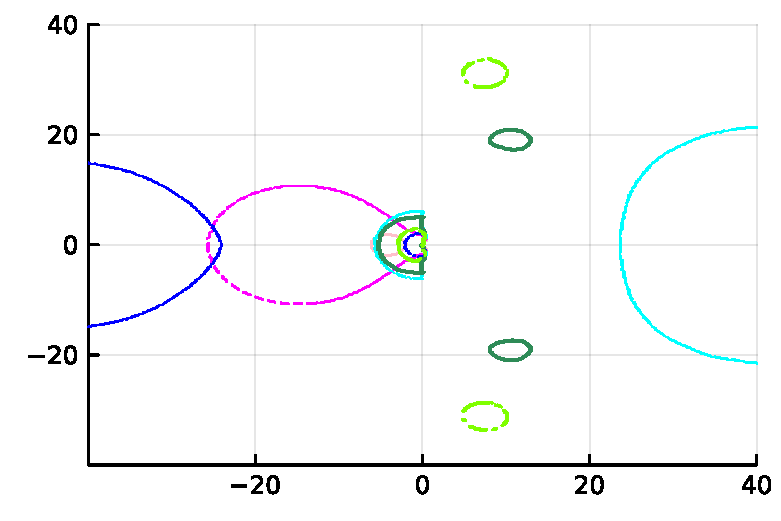
\includegraphics[width=\textwidth]{pdf/odepics/ImExD1_IMEXDeC_subtimesteps_equispaced_range=40.pdf}
%		\centerline{equispaced nodes}
%	\end{minipage}
%	\begin{minipage}[t]{0.45\textwidth}
%		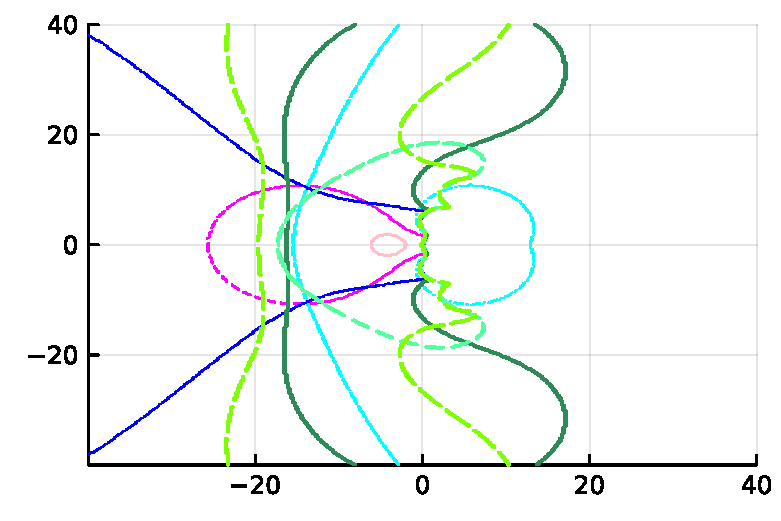
\includegraphics[width=\textwidth]{pdf/odepics/ImExD1_IMEXDeC_subtimesteps_gaussLobatto_range=40.pdf}
%		\centerline{Gauss-Lobatto nodes}
%	\end{minipage}
%	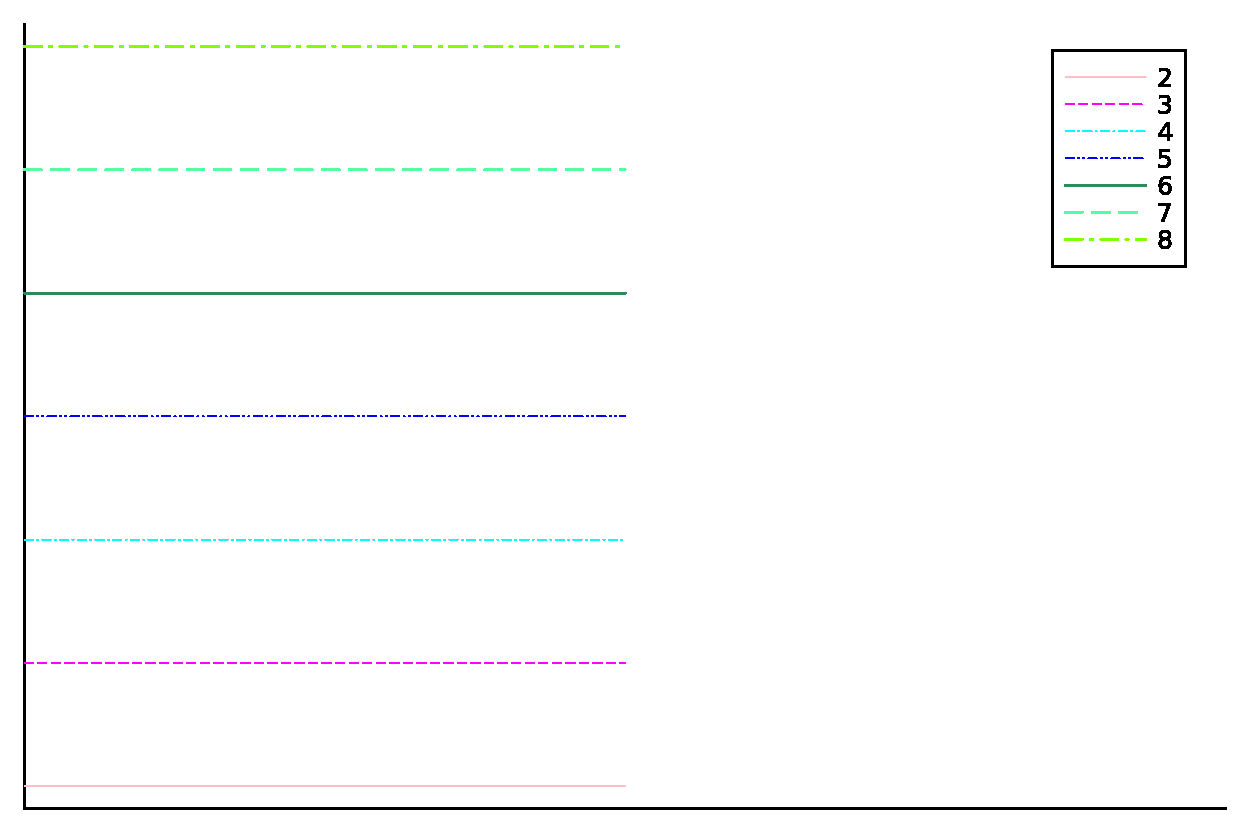
\includegraphics[width=0.08\textwidth, trim={491 180 30 23}, clip]{pdf/odepics/colors_a-d_new_2-8_no_order.pdf}
%	\caption{$\mathcal{D}_1$ Stability Region for IMEX sDeC: orders 2 to 8}
%\label{fig: HundsdorferD1_IMEXsDeC}
%\end{figure}
In Figure~\ref{fig: HundsdorferD1_IMEX} (right), we show the results for the IMEX ADER methods. 
We note that most of the methods fulfill nearly A-stability by almost covering the negative half-plane. %, but most of it except for relatively small, limited sets. 
We highlight that for the equispaced case we do not show the full outreach of the stability regions. 
While in most of the cases, for the almost A-stable cases, these contour lines represent the inner bounds of unlimited stability regions, in the cases of order 5 and 8 we just have large, limited stability regions, as we also could observe for example in the $\mathcal{D}_1$ IMEX DeC case for equispaced nodes. 
Therefore, it seems like we can not guarantee this almost A-stability for the IMEX ADER, but just for some of the orders of accuracy.
%\begin{figure}
%	\centering
%	\begin{minipage}[t]{0.45\textwidth}
%		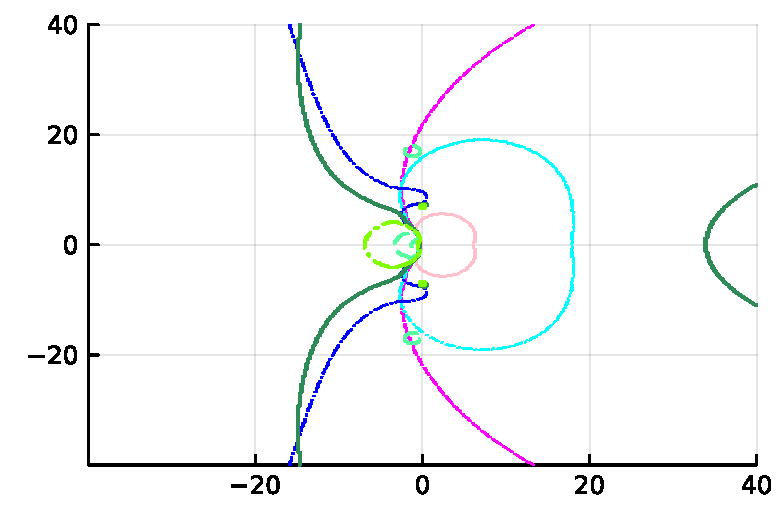
\includegraphics[width=\textwidth]{pdf/odepics/ImExD1_IMEXADER_equispaced_range=40.pdf}
%		\centerline{equispaced nodes}
%	\end{minipage}
%	\begin{minipage}[t]{0.45\textwidth}
%		\includegraphics[width=\textwidth]{pdf/odepics/ImExD1_IMEXADER_gaussLobatto_range=40.pdf}
%		\centerline{Gauss-Lobatto nodes}
%	\end{minipage}
%	\includegraphics[width=0.08\textwidth, trim={491 180 30 23}, clip]{pdf/odepics/colors_a-d_new_2-8_no_order.pdf}
%	\caption{$\mathcal{D}_1$ Stability Region for IMEX ADER: orders 2 to 8}
%\label{fig: HundsdorferD1_IMEXADER}
%\end{figure}

%Remark that for the $\mathcal{D}_0$ case, an order of magnitude of the explicit Euler stability region can be considered as good as it gets controlled by the non-stiff term, while for the $\mathcal{D}_1$ case A-stability would be desired due to stiffness. 
Therefore, we can conclude, that some of the IMEX ADER stability regions cover the areas in the complex plane, that we assumed for a stable method in the context of $\mathcal{D}_0$ and $\mathcal{D}_1$, while the DeC and sDeC methods have their limitations with $\mathcal{D}_0= \emptyset$ in every case and bounded stability regions for most of the cases in the scope of $\mathcal{D}_1$. Nevertheless, we need to keep in mind that the set conditions are very strict, so,  the methods might still be applicable to some stiff equations. % \\
These results reflect what we have seen for the respective implicit methods.


	\section{PDE: analysis of advection-diffusion}
	\label{sec: advection_diffusion}
	In this section, we want to extend our stability analysis to the one-dimensional advection-diffusion equation
\begin{equation}\label{eq: A-D_equation}
u_t(x,t) + au_x(x,t) = du_{xx}(x,t), \quad a\ge0, \ d \ge 0, \qquad x \in \Omega \subset \mathbb R,
\end{equation}
where $a$ is the coefficient of the advection term and $d$ the coefficient of the diffusion term, using the von  \PO{Neumann stability analysis}. %principles.
\PO{After the space discretization, we discretize the advection part with an explicit time-integration scheme and the diffusion with an implicit one}.
The linear stability of the DeC method in PDE contexts was studied for explicit methods for advection equations with FEM spatial discretizations and various stabilization techniques in \cite{michel2021spectral,michel2023spectral}, while in the IMEX context for FEM methods applied to kinetic models in \cite{torlo2020hyperbolic}.
For the ADER method, a von Neumann stability analysis was applied to the original formulation \cite{titarev2007analysis,dematte2020ader}, but not on the modern version that we are studying. \PO{We close this gap with our investigation in the following.}
\subsection{Finite Difference discretization}
\label{sec: spatial_discretization}
We apply spatial discretizations to the spatial derivative operators, namely $\partial_x$ and $\partial_{xx}$. 
We consider a uniformed grid $\Omega_{\Delta x}=\left\{x_j \ : \ x_j = x_0 + j\Delta x, \ j \in \{0,\hdots , J\}\right\}$ with periodic boundary conditions and we denote the approximation of $u(x_j)=u(x_j,t)$ by $w_j$.

To discretize the advection term in \eqref{eq: A-D_equation}, i.e. the first spatial derivative $\partial_xu(x)$, we make usage of the stable finite difference stencils introduced in \cite{Iserles1982}. Assume we discretize $\partial_xu$ at $x_j$ by an $[r,s]$-discretization
\begin{equation}\label{eq: r-s_scheme}
\partial^{[r,s]}_{\Delta x}(u(x_j)) = \frac{1}{\Delta x} \sum\limits_{k=-r}^s \alpha_k w_{j+k},
\end{equation}
with $r,\ s$ such that $\alpha_{j-r}, \alpha_{j+s} \neq 0$.
The maximum order we can achieve with an $[r,s]$- discretization is $q=r+s$ and this discretization actually reaches order $q$ and is unique by setting the coefficients in \eqref{eq: r-s_scheme} as
	\begin{align}\label{eq:def_advection_optimal_stencil}
	\alpha_0&=
	\begin{cases}
	\sum\limits_{k=r+1}^s\frac{1}{k}, & s\ge r+1, \\
	0, & s=r, \\
	\sum\limits_{k=s+1}^r\frac{1}{k}, & r\ge s+1, 
	\end{cases} \qquad
	\alpha_k = \frac{(-1)^{k+1}}{k}\cdot \frac{r!s!}{(r+k)!(s-k)!}, \quad -r\le k \le s, \ k\neq0.
	\end{align}
 It is also proven in \cite{Iserles1982} that these so-called $\textit{optimal-order}$ schemes of order $q$ are stable if and only if $s\le r \le s+2$ for $a>0$.\\
We  involve these stable $\textit{optimal-order}$ schemes into our analysis. 
We introduce upwinding in the choice of the stencils, in particular, we will consider $[r, r +1]$ stencils for odd optimal-order scheme and $[r, r+2]$ stencils for an even optimal-order scheme for the advection part.

For the diffusion term, we will just use a central finite difference discretization of the second spatial derivative $\partial_{xx} u(x)$ given in Table~\ref{tab: CFD-schemes_first_deriv}.
\begin{table}
	\centering
	\caption{Central finite difference discretizations of $\partial_{xx}$ applied onto $w$ centered in $j$  \cite{fornberg_finite_difference}}
	\label{tab: CFD-schemes_first_deriv}
	\small
	\begin{tabular}[h]{|c|c|}
		\hline
		order & finite difference for $\partial_{\Delta x}^2(u(x_j))$\\
		\hline
		2 & $\frac{1}{\Delta x^2}\left(w_{j-1}-2w_j+w_{j+1}\right)$\\
		\hline
		4 & $\frac{1}{\Delta x^2}\left( -\frac{1}{12}w_{j-2} +\frac{4}{3}w_{j-1} -\frac{5}{2}w_j   +\frac{4}{3}w_{j+1}  -\frac{1}{12}w_{j+2}\right)$\\
		\hline
		6 & $\frac{1}{\Delta x^2}\left(\frac{1}{90}w_{j-3} - \frac{3}{20}w_{j-2} + \frac{3}{2}w_{j} - \frac{49}{18}w_{j} + \frac{3}{2}w_{j} - \frac{3}{20}w_{j+2} + \frac{1}{90}w_{j+3}\right)$\\
		\hline
		8 & $\frac{1}{\Delta x^2}\left(
		-\frac{1}{56}w_{j-4} + \frac{1}{420}w_{j-3} - \frac{1}{5}w_{j-2} + \frac{8}{5}w_{j-1} - \frac{205}{72}w_{j} + \frac{8}{5}w_{j+1} - \frac{1}{5}w_{j+2} + \frac{1}{420}w_{j+3} - \frac{1}{56}w_{j+4}
		\right)$\\
		\hline
	\end{tabular}
\end{table}

\subsection{von Neumann analysis}
\label{sec: stability_theory_PDE}
To analyze the stability of the described methods, we make use of the von Neumann stability analysis for linear partial differential equations \cite{leveque2007finite}.
%\subsubsection{von Neumann Stability}
Briefly summarized, we investigate the behavior inside the numerical scheme of the Fourier modes
\begin{equation}\label{eq: fourier_modes}
w^n_j = v^ne^{ikx_j},
\end{equation}
where $w^n_j$ is the discretization of $u(x_j, t_n)$ and $k$ is the wavenumber and we focus on the representation coefficient $v^n$. 
Indeed, $e^{ikx}$ are eigenfunctions of the differential operator $\partial_x$ and therefore for any linear differential operator. 
If we use \eqref{eq: fourier_modes} in our discretized system, we obtain a system of the form
\begin{equation}
\label{eq: ampfactor}
v^{n+1}=G(k, \Delta x, \Delta t, a, d)v^n.
\end{equation}
with the amplification factor $G\in \mathbb{C}$ independent on the mesh point $x_j$.
%Now, to check the stability of the scheme, we need that $\lvert{v^{n+1}}\rvert= \lvert{G(k, \Delta x, \Delta t, a, d)v^n}\rvert \leq \lvert v^n\rvert$. 
\PO{Stability means in our context that $\lvert{v^{n+1}}\rvert= \lvert{G(k, \Delta x, \Delta t, a, d)v^n}\rvert \leq \lvert v^n\rvert$ holds.}
In practice, we check that $\lvert G (k, \Delta x, \Delta t, a, d) \rvert \le 1$. \PO{This implies stability for the related method and due to the  Lax-Richtmeyer theorem \cite{leveque2007finite} convergence can be ensured.}
Note that for consistency, we included the parameters $a$ and $d$ into the dependency of $G$ to cover all advection-diffusion equations. \\
% This theory concludes in the following condition: 
%\begin{prop}\textbf{Richtmyer condition}\\
%	A finite difference scheme equipped with a time-stepping method is stable in the stability area $\Lambda$ if and only if there exists a constant $K$, such that
%	\begin{equation*}
%	\lvert G (k, \Delta x, \Delta t, a, d) \rvert \le 1+ K \Delta t
%	\end{equation*}
%	with $(k, \Delta x, \Delta t, a, d)\in \Lambda$. 
%\end{prop}
%Remark that for consistency, we included the parameters $a$ and $d$ into the dependency of $G$ to cover all advection-diffusion equations. When we evaluate the amplification factors numerically later on, we will probe the slightly more strict von Neumann condition $\lvert G (k, \Delta x, \Delta t, a, d) \rvert \le 1$ for stability. \\
%This whole analysis gains its relevance based on the following statement.
%\begin{theorem}\textbf{Lax-Richtmyer}\\
%	A consistent finite difference scheme for a partial differental equation with a well-posed inital value problem is convergent if and only if its stable.
%\end{theorem}
%%%%%%%%%%%%%%%%%
%Displaying Stability
%%%%%%%%%%%%%%%%%
Typically, in order to estimate the stability of the advection-diffusion equation, an analytical study of $G$ in all the parameters should be performed. 
This is not feasible when considering high order schemes as ADER and DeC.
Hence, we will evaluate the amplification factor numerically, similarly to what we did with the stability functions in the ODE case.

Before running all the simulations, we need to understand what are the free variables of the function $G$. First of all, the wavenumbers  should be bounded $k \in \lbrace -n_0-1 , \dots, n_0+1 \rbrace \subset \mathbb Z$ and the maximum wavenumber $n_0+1$ is strongly related with the discretization scale $\Delta x$. Indeed, by  Nyquist–Shannon sampling theorem, only functions with frequency less than $\frac{|x_J-x_0|}{2\Delta x}$ can be represented on our discretization. Hence, we will choose $n_0=10^3$ to take in consideration fine grids.

Then, we have further variables $a,d,\Delta x,\Delta t $ that are often coupled together: in the advection term ($a\Delta t/\Delta x$) and in the diffusion term ($d\Delta t/\Delta x^2$). We keep this in mind when studying the behavior of $G$, as we can recast few methods to the same coefficients.

\subsubsection{Displaying stability}
It is stated and numerically shown in \cite{TanChenShu_ImEx_Stability, WangShuZhang_LDG1_2015,WangShuZhang_LDG_2016} that several schemes as the local discontinuous Galerkin scheme \cite{WangShuZhang_LDG1_2015,WangShuZhang_LDG_2016} and other finite difference schemes combined with an IMEX RK method are stable if the time step is upper bounded by some $\tau_0$. This $\tau_0$ is proportional to $\frac{d}{a^2}$, i.e., if $\Delta t\le\tau_0= E_0\cdot \frac{d}{a^2}$ for some $E_0>0$.
%%%%%%%%%%%%%%%%%
%C, D, E Approach
%%%%%%%%%%%%%%%%%
Considering the before mentioned parameters $\Delta x, \Delta t, a,d$, we introduce two new coefficients
\begin{equation}
C=\frac{a\Delta t}{\Delta x}, \quad D=\frac{d\Delta t}{{(\Delta x)}^2}.
\end{equation}

Moreover, using the coefficients $C$ and $D$ reveals an equivalent condition to \cite{TanChenShu_ImEx_Stability}, if we assume that the quotient
\begin{equation*}
E:=\frac{C^2}{D}= \frac{ \Delta t ^2 a^2 }{\Delta x^2} \frac{\Delta x^2}{d \Delta t} = \frac{a^2}{d}\Delta t
\end{equation*}
is bounded by some constant $E_0$, indeed,
\begin{equation*}
E= \frac{a^2}{d}\Delta t\le E_0 \quad \Longleftrightarrow \quad \Delta t \le E_0 \cdot \frac{d}{a^2}=\tau_0.
\end{equation*}
Therefore, for a given method solving the advection-diffusion equation, we can rewrite the amplification factor  with \eqref{eq: ampfactor} as
\begin{equation}
	g(k,C,E)=G(k,\Delta x, \Delta t, a,d).
\end{equation}

\begin{definition}[Scheme notation]	\label{defi: notation_pde_method}
	To shorten the notation, we denote the considered method for the advection-diffusion equation by $[\TMM,\NODES,N, A_n,D_m],$ where
	\begin{itemize}
		\item $\TMM$ stands for the respective IMEX time-marching method, i.e. $\DeC$, $\ADER$, $\sDeC$,
		\item $\NODES$ stands for the used quadrature nodes for the \TMM, i.e. {\eq} or $\GLB$,
		\item $N$ stands for the order of the considered time-marching method $\TMM$,
		\item $A_n$ denotes the optimal first derivative stencil of order $n$ defined in \eqref{eq:def_advection_optimal_stencil} used for the advection term,
		\item $D_m$ denotes the central second derivative stencil of order $m$ in Table~\ref{tab: CFD-schemes_first_deriv} used for the diffusion term.
	\end{itemize}
\end{definition}


\begin{remark}
	With the previous plots, we recognize two sufficient conditions to obtain stability:
	\begin{itemize}
		\item the well known CFL-condition, i.e., if $C$ is lower than some constant $C_0$ only dependent on the method, then the method is stable.
		\item the new numerically obtained condition, designated as the $E_0$-condition: If $E$ is lower than some constant $E_0$ dependent on the method, then the method is stable.
	\end{itemize}
	
	These two parameters $C$ and $E$ include all the remaining ones and show therefore a full picture.
\end{remark}

As we can see in Figure~\ref{fig: exa_ImExDeC3_diff2_adv1}, the unstable area of this specific method seems to be bounded by the linear constraints $C\geq C_0$ and $E\geq E_0$. We will observe numerically that these unstable regions are indeed similarly bounded in most of our methods.
\begin{definition}[Stability parameters $C_0$ and $E_0$]
	Given the amplification factor $g(k,C,E)$ of a discretization of the advection-diffusion equation, we define the two stability parameters $C_0$ and $E_0$ by
	\begin{itemize}
		\item $C_0:=\max_{C\in \mathcal{S}} C$ with $\mathcal{S}=\lbrace C: \lvert g(k,C,E)\rvert \leq 1, \, \forall E>0, \,\forall k \in [-n_0-1,n_0+1] \rbrace$,
		\item $E_0:=\max_{E\in \mathcal{R}}E$ with $\mathcal{R}= \lbrace E: \lvert g(k,C,E)\rvert \leq 1,\, \forall C>0,\,\forall k \in [-n_0-1,n_0+1]\rbrace .$
	\end{itemize}
\end{definition}
Therefore, the strategy we want to follow is to look at the areas of stability by evaluating the amplification factor $\max_k |g(k,C,E)|$ like in Figure~\ref{fig: exa_ImExDeC3_diff2_adv1} and numerically calculating the parameters $C_0$ and $E_0$ for our methods, when possible.

Note, that the condition $E<E_0$ does not depend on $\Delta x$ and avoids CFL restrictions. We should always keep in mind that our numerical evaluations can just cover finite ranges of $C$ and $E$. 
Hence, we checked that the displayed limits for $E$ and $C$ are actually bounds also for larger domains of $C$ and $E$.
Moreover, we also observed that the considered results do not vary much for large values of $n_0$, hence, we set $n_0=10^3$. Due time-efficiency, we will use this value for every evaluation in the von Neumann stability analysis context for the rest of this work. Further, all plots in this section will be evaluated and displayed at $400\times 400$ grid points.
\subsubsection{Numerical analysis}
%To distinguish the different orders, we use different colors to the  bounds according to the legend figure~\ref{fig: legend_a-d}. 
In the following plots, we remark that the colors are assigned to different orders, indeed, we will vary alternatively the order of the advection method, of the time-marching, of the diffusion method or of all of them. We will specify for each plot what is the object of the study.
%\begin{figure}
%	\centering
%	\includegraphics[width=0.17\textwidth, trim={461 256 30 23}, clip]{pdf/odepics/colors_a-d_new_1-8.pdf}
%	\caption{Legend for the different orders.}
%	\label{fig: legend_a-d}
%\end{figure}

We start by varying only the time scheme order. 
In Figure~\ref{fig: grp_adv1_diff2}, the stability areas of several methods are shown, i.e., $[\TMM,\NODES,k, A_1,D_2]$ varying the time scheme and the nodes. 
As in Figure~\ref{fig: exa_ImExDeC3_diff2_adv1}, the plotted lines separates the stable region in the lower left part from the unstable region in the upper right side of the $C$-$E$ plane. 
We see a similar behavior for mostly all methods. 
Increasing the order of the time marching method results in a larger stability region and in larger values for $E_0$ and $C_0$. 

\begin{figure}
	\centering
	\includegraphics[width=0.5\textwidth,trim={160 340 30 22}, clip]{pdf/pdepics/legends/colors_a-d_new_horiz_2-8_no_order.pdf}\\	\begin{minipage}[t]{0.32\textwidth}
		\includegraphics[width=\textwidth]{pdf/pdepics/diff/IMEXDeC_equispaced_TMM_ord_2-8.pdf}
		\centering
		IMEX DeC eq
	\end{minipage} 
	\begin{minipage}[t]{0.32\textwidth}
		\includegraphics[width=\textwidth]{pdf/pdepics/diff/IMEXDeC_subtimesteps_equispaced_TMM_ord_2-8.pdf}
		\centering
		IMEX sDeC eq
	\end{minipage}
	\begin{minipage}[t]{0.32\textwidth}
		\includegraphics[width=\textwidth]{pdf/pdepics/diff/IMEXADER_equispaced_TMM_ord_2-8.pdf}
		\centering
		IMEX ADER eq
	\end{minipage} \\
	\begin{minipage}[t]{0.32\textwidth}
		\includegraphics[width=\textwidth]{pdf/pdepics/diff/IMEXDeC_gaussLobatto_TMM_ord_2-8.pdf}
		\centering
		IMEX DeC GLB
	\end{minipage} 
	\begin{minipage}[t]{0.32\textwidth}
		\includegraphics[width=\textwidth]{pdf/pdepics/diff/IMEXDeC_subtimesteps_gaussLobatto_TMM_ord_2-8.pdf}
		\centering
		IMEX sDeC GLB
	\end{minipage}
	\begin{minipage}[t]{0.32\textwidth}
		\includegraphics[width=\textwidth]{pdf/pdepics/diff/IMEXADER_gaussLobatto_TMM_ord_2-8.pdf}
		\centering
		IMEX ADER GLB
	\end{minipage} 
	\caption{Stability areas for $[\TMM,\NODES,k, A_1,D_2]$ for $\TMM$ as IMEX DeC (left), IMEX sDeC (center) and IMEX ADER (right) with eq (top) and GLB (bottom) nodes: $\TMM$ order $k$ from 2 to 8}
	\label{fig: grp_adv1_diff2}
\end{figure}

In the equispaced case we do not observe major differences for the DeC and sDeC methods, 
while, for the ADER cases, the usage of equispaced nodes results in an irregular reduction to $C_0=0$ for some orders (7 and 8), meaning that we can not assure stability as we did in the other cases for high order methods. 
This is probably impacted by the catastrophic cancellation which occurs in Newton-Cotes quadratures with more than 8 points that occur for orders larger than $6$, used in the considered IMEX ADER method. 
%The reason for this catastrophic cancellation effect lies in negative weights of the quadrature which firstly appear for 8 steps. 
%This hypothesis is also supported by the IMEX ADER in figure~\ref{fig: grp_adv1_diff2_GLB} with Gauss-Lobatto nodes, where this phenomenon does not appear.
For this reason, we will mainly analyze this method with Gauss-Lobatto nodes for the other cases.



In Figure~\ref{fig: exa_advterm}, we display the stability areas for the $[\DeC,\eq,8, A_k,D_2]$, $[\sDeC,\eq,8, A_k,D_8]$ and $[\ADER,\GLB,8, A_k,D_8]$ increasing the order for the finite difference scheme for the advection operator. 
For DeC (left), this does not lead to higher values for $E_0$ or $C_0$, but seemingly decreases for odd orders and increases for even orders, while starting with relatively big values for order 1 and relatively small values for order 2. 
It seems that they all guide towards a specific border line. It is also surprising that  we do not get a border $E_0>0$ for order 6 in the advection term for equispaced nodes, while we do for GLB ones (not displayed). 
These phenomena hold for all remaining combinations of time-marching methods, respective orders and nodes also, i.e. if we increase the order of the diffusion term, we can eliminate instabilities that occur due to the advection term, while the remaining variables just play a minor role. 
Exemplary, we display in Figure~\ref{fig: exa_advterm} on the right the $[\ADER,\GLB,8, A_k,D_2]$  to underline this statement. 
This is again not true for order 6 for which all time methods do not show a stability region of type $E\leq E_0$.
%The only exception we observed appears for the higher order ADER with equispaced nodes, as we already saw in figure \ref{fig: grp_adv1_diff2_eq} and is displayed for varying advection terms in figure \ref{fig: exa_advtermADER} on the right: Under these conditions, the instabilities remain.
\begin{figure}[!h]
	\centering
	\includegraphics[width=0.6\textwidth,trim={100 340 30 22}, clip]{pdf/pdepics/legends/colors_a-d_new_horiz_1-8_no_order.pdf}\\
	\begin{minipage}[t]{0.32\textwidth}
		\includegraphics[width=\textwidth]{pdf/pdepics/diff/IMEXDeC_equispaced_adv_ord_1-8.pdf}
		\centering
		$[\DeC,\eq,8, A_k,D_2]$
	\end{minipage} 
	\begin{minipage}[t]{0.32\textwidth}
		\includegraphics[width=\textwidth]{pdf/pdepics/diff/IMEXDeC_subtimesteps_equispaced_adv_ord_1-8.pdf}
		\centering
		$[\sDeC,\eq,8, A_k,D_2]$
	\end{minipage}
	\begin{minipage}[t]{0.32\textwidth}
		WAITING FOR PLOT!
		%\includegraphics[width=\textwidth]{pdf/pdepics/diff/IMEXADER_equispaced_adv_ord_1-8.pdf}
		\centering
		$[\ADER,\eq,8, A_k,D_2]$
	\end{minipage}\\
	\begin{minipage}[t]{0.32\textwidth}
		\includegraphics[width=\textwidth]{pdf/pdepics/diff/IMEXDeC_gaussLobatto_adv_ord_1-8.pdf}
		\centering
		$[\DeC,\GLB,8, A_k,D_2]$
	\end{minipage}
	\begin{minipage}[t]{0.32\textwidth}
		\includegraphics[width=\textwidth]{pdf/pdepics/diff/IMEXDeC_subtimesteps_gaussLobatto_adv_ord_1-8.pdf}
		\centering
		$[\sDeC,\GLB,8, A_k,D_2]$
	\end{minipage}
	\begin{minipage}[t]{0.32\textwidth}
		\includegraphics[width=\textwidth]{pdf/pdepics/diff/IMEXADER_gaussLobatto_adv_ord_1-8.pdf}
		\centering
		$[\ADER,\GLB,8, A_k,D_2]$
	\end{minipage}
	\caption{DeC Stability areas varying the order of the advection method}
	\label{fig: exa_advterm}
\end{figure}


In Figure~\ref{fig: exa_diffterm}, we show the stability regions increasing the order of the diffusion operator for $[\TMM,eq, 8, A_1,D_k]$, where $\TMM$ is every of the 3 considered methods and $k \in \{2,4,6,8\}$.  We observe that the stability areas of all methods vary slightly, but do not increase or decrease the stability region in a significant way.

\begin{figure}[!h]
	\centering
	\includegraphics[width=0.6\textwidth,trim={160 340 30 22}, clip]{pdf/pdepics/legends/colors_a-d_new_horiz_2-8_no_order.pdf}\\
	\begin{minipage}[t]{0.32\textwidth}
		\includegraphics[width=\textwidth]{pdf/pdepics/diff/IMEXDeC_equispaced_diff_ord_2468.pdf}
		\centering
		$[\DeC,\eq, 8, A_1,D_k]$
	\end{minipage} 
	\begin{minipage}[t]{0.32\textwidth}
		\includegraphics[width=\textwidth]{pdf/pdepics/diff/IMEXDeC_subtimesteps_equispaced_diff_ord_2468.pdf}
		\centering
		$[\sDeC,\eq, 8, A_1,D_k]$
	\end{minipage}
	\begin{minipage}[t]{0.32\textwidth}
		WAITING FOR PLOT
		%\includegraphics[width=\textwidth]{pdf/pdepics/diff/IMEXADER_equispaced_diff_ord_2468.pdf}
		\centering
		$[\ADER,\eq, 8, A_1,D_k]$
	\end{minipage}\\
	\begin{minipage}[t]{0.32\textwidth}
		\includegraphics[width=\textwidth]{pdf/pdepics/diff/IMEXDeC_gaussLobatto_diff_ord_2468.pdf}
		\centering
		$[\DeC,\GLB, 8, A_1,D_k]$
	\end{minipage} 
	\begin{minipage}[t]{0.32\textwidth}
		\includegraphics[width=\textwidth]{pdf/pdepics/diff/IMEXDeC_subtimesteps_gaussLobatto_diff_ord_2468.pdf}
		\centering
		$[\sDeC,\GLB, 8, A_1,D_k]$
	\end{minipage}
	\begin{minipage}[t]{0.32\textwidth}
		\includegraphics[width=\textwidth]{pdf/pdepics/diff/IMEXADER_gaussLobatto_diff_ord_2468.pdf}
		\centering
		$[\ADER,\GLB, 8, A_1,D_k]$
	\end{minipage}
	\caption{Stability areas varying the order of the diffusion method}
	\label{fig: exa_diffterm}
\end{figure}
\todo{The following paragraph would be rewritten shortly. There do not happen many new interesting things, just showing it works, giving a hint to the table and reminding that the instabilities for advection order 6 gets removes by matching the dispersion order}
In Figure~\ref{fig: exa_difftermsim}, we study the space--time discretizations matching the orders of the time scheme with the order of the spatial terms, i.e.  $[\TMM,\GLB, k, A_k,D_{2\lceil k/2 \rceil}]$, where $\TMM$ is one of the 3 considered methods and $k \in \{2, \hdots, 8\}$.
Here, we can observe for all cases that the higher order terms results in slightly larger stability areas and also in bigger $C_0$ and $E_0$, which leads us to the behavior we have already seen in Figure~\ref{fig: grp_adv1_diff2} varying only the order of the time scheme. 

\begin{figure}[!h]
	\centering
	\includegraphics[width=0.6\textwidth,trim={160 340 30 22}, clip]{pdf/pdepics/legends/colors_a-d_new_horiz_2-8_no_order.pdf}\\
	\begin{minipage}[t]{0.32\textwidth}
		\includegraphics[width=\textwidth]{pdf/pdepics/diff/IMEXDeC_equispaced_all_2-8.pdf}
		\centering
		$[\DeC,\eq, k, A_k,D_{2\lceil k/2 \rceil}]$
	\end{minipage} 
	\begin{minipage}[t]{0.32\textwidth}
		\includegraphics[width=\textwidth]{pdf/pdepics/diff/IMEXDeC_subtimesteps_equispaced_all_2-8.pdf}
		\centering
		$[\sDeC,\eq, k, A_k,D_{2\lceil k/2 \rceil}]$
	\end{minipage}
	\begin{minipage}[t]{0.32\textwidth}
		\includegraphics[width=\textwidth]{pdf/pdepics/diff/IMEXADER_equispaced_all_2-8.pdf}
		\centering
		$[\ADER,\eq, k, A_k,D_{2\lceil k/2 \rceil}]$
	\end{minipage}\\
	\begin{minipage}[t]{0.32\textwidth}
		\includegraphics[width=\textwidth]{pdf/pdepics/diff/IMEXDeC_gaussLobatto_all_2-8.pdf}
		\centering
		$[\DeC,\GLB, k, A_k,D_{2\lceil k/2 \rceil}]$
	\end{minipage} 
	\begin{minipage}[t]{0.32\textwidth}
		\includegraphics[width=\textwidth]{pdf/pdepics/diff/IMEXDeC_subtimesteps_gaussLobatto_all_2-8.pdf}
		\centering
		$[\sDeC,\GLB, k, A_k,D_{2\lceil k/2 \rceil}]$
	\end{minipage}
	\begin{minipage}[t]{0.32\textwidth}
		\includegraphics[width=\textwidth]{pdf/pdepics/diff/IMEXADER_gaussLobatto_all_2-8.pdf}
		\centering
		$[\ADER,\GLB, k, A_k,D_{2\lceil k/2 \rceil}]$
	\end{minipage}	
	\caption{Stability areas varying the order of all partial methods.}
	\label{fig: exa_difftermsim}
\end{figure}

We can conclude that increasing the order of the time-marching method results in higher values for both $C_0$ and $E_0$. However, the here considered higher order finite differences for the spatial discretizations do not grant significant improvements. In the recent analysis, the border $E_0$ vanishes for the special setting IMEX ADER of order $>7$  with equispaced nodes, independently of the spatial discretization we used. We also get this phenomenon by setting the advection stencil to order 6, but this problem can be overcome by the usage of high order diffusion stencils.\\
Remark also, that there are plenty more options to test, which we leave out because of space restrictions. Nevertheless, we presented all remarkable combinations of methods we tested and a summary of their results.

\begin{table}
	\centering
	\caption{Approximated border values $C_0$ (up to 2 decimals) and $E_0$ (up to 1 decimal) for Gauss--Lobatto methods with operators with optimal order $k$}\label{tab:CE_values}
	\begin{tabular}{|c||c|c||c|c||c|c|}\hline
				$k$&
		\multicolumn{2}{|c||}{$[\DeC,\GLB,k,A_k,D_{2\lceil k/2 \rceil}]$}&
		\multicolumn{2}{|c||}{$[\sDeC,\GLB,k,A_k,D_{2\lceil k/2 \rceil}]$}&
		\multicolumn{2}{|c|}{$[\ADER,\GLB,k,A_k,D_{2\lceil k/2 \rceil}]$}\\\hline
		&$\qquad C_0\qquad$&$E_0$&$\qquad C_0\qquad$&$E_0$&$\qquad C_0\qquad$&$E_0$\\\hline
		2& 0.50 &2.5&0.50&2.5&0.50&0.7\\
		3& 1.63 &6.1&1.69&5.1&1.63&4.5\\
		4& 1.04&6.9&1.43&4.9&1.04&4.2\\
		5& 1.74&8.8&2.31&6.6&1.74&7.2\\
		6& 1.60&4.1&2.33&4.2&1.60&4.1\\
		7& 1.94&9.5&3.12&7.5&1.94&8.5\\
		8&2.00&10.2&2.85&5.9&2.00&9.8\\ \hline
	\end{tabular}
\end{table}

In Table~\ref{tab:CE_values}, we study the operators with order $k$ matching for the time and spatial discretization for time schemes defined by GLB nodes. We display in that table the maximal values $C_0$ and $E_0$. 
We clearly see that they increase as the order increases. 
The only value that is not uniform among the methods is $E_0$ for ADER GLB of order 2, for which we have a restrictive bound.
We also want to highlight, that $C_0$ matches inbetween the DeC and ADER methods for the same orders. This is probably due to their coinciding explicit stability regions for ODEs, as pointed out in \cite{Han_Veiga_2021}. 
	
	\section{PDE: analysis of advection-dispersion}
	\label{sec:PDE_adv_disp}
	In this section, we extend the analysis and results to observe the behavior of IMEX ADER and DeC methods onto the advection-dispersion equation
\begin{equation}
\label{eq: A-Disp_equation}
u_t(x,t) + au_x(x,t) + \beta u_{xxx}(x,t) = 0, \quad a\ge0, \ \beta \ge 0.
\end{equation}
\subsection{FD discretization}
\label{sec: disp_spatial_discretization}
First, we  introduce at this point the considered spatial discretizations for the advection-dispersion equation. Thereby, we consider the same discretization for the advection term, as introduced in Section~\ref{sec: spatial_discretization}.

For the dispersion term, we will take two different types of methods into account: Central finite difference and upwind schemes. The underlying theory and assumptions are the same as we saw previously and their orders can be proven analogously. We consider the following central finite difference scheme of order $2$ 
\begin{equation}
	\label{eq: CFD-schemes_third_deriv}
	B_2: \qquad\partial_{\Delta x}^3(u(x_j)) = \frac{1}{{\Delta x}^3}\left(-\frac{1}{2}w_{j-2} + w_{j-1} - w_{j+1} + \frac{1}{2}w_{j+2}\right)
\end{equation}
and the upwind scheme used in \cite{TanChenShu_ImEx_Stability} to test stability for the advection-dispersion equation \eqref{eq: A-Disp_equation}. It is of order 3 and given by
\begin{equation}
\label{eq: shu_upwind_dispersion}
B_3: \qquad\partial_{\Delta x}^3(u(x_j)) =\frac{1}{4{\Delta x}^3}\left( -w_{j-2} - w_{j-1}  + 10w_{j} - 14w_{j+1} + 7w_{j+2} - w_{j+3}\right).
\end{equation}
For higher orders, we have used the optimal $2r+1$ order formula on stencils of the type $[-r,r+1]$ with the tool provided in \cite{fdcc} and we denote them by $B_{2r+1}$. In Figure~\ref{fig:eig_disp}, the Fourier value of these dispersion operators are shown. We do not plot $B_2$ that lies on the imaginary axis. 
\begin{figure}
	\centering
	\includegraphics[width=0.39\textwidth]{pdf/pdepics/disp/eig_disp_oper_all.pdf}
	\caption{Fourier coefficient of the dispersion operators $B_{2r+1}$ varying the Fourier mode.}\label{fig:eig_disp}
\end{figure}
\subsection{von Neumann analysis}
As previously done for the advection--diffusion problem, we will perform the von Neumann analysis by looking at the coefficients of the finite difference schemes, i.e.,
$$C=a\frac{\Delta t}{\Delta x},\qquad P= \beta\frac{\Delta t}{{\Delta x}^3}.$$
The procedure is analogous to the advection--diffusion one, with $C,\,P$ instead of $C,\,E$.
%So technically, we compute the methods in the same way and just adapt the spatial schemes from the diffusion term to the dispersion term. Remark that also the sign of this term changes. 
\subsubsection{Displaying stability}
To denote the considered methods, we use again the notation introduced for the advection-diffusion equation
	\begin{equation*}
[\TMM,\NODES,N, A_n,B_m],
\end{equation*}
where $B_m$ refers to the upwind $m$-th order stencils of type $[-r,r+1]$.
We proceed evaluating the amplification factor 
\begin{equation*}
G(k,\Delta x, \Delta t, a, \beta)=g(k,C,P)
\end{equation*}
to observe the stability region as a function of $C$ and $P$. 
In opposition to the advection--diffusion case, in \cite{TanChenShu_ImEx_Stability} only a CFL condition is found, even if, numerically, they observe larger stability regions with a little of dispersion.
We want to give a more comprehensive study of this behavior for different schemes and, as before, we look for meaningful coefficients that bounded by some constants give the stability. 
To find such coefficients, we proceed with an example.
\begin{example}\label{exa: disp_displaying_stability}
	In Figure~\ref{fig: disp_IIMEXDeC2/3} we display the stability areas for the $[\DeC, \eq,2,A_1, B_2]$ and $[\DeC, \eq,3,A_1, B_2]$ on the $(C,P)$ plane (left).
	In the IMEXDeC2 case, we note that for low $P$ a CFL constraint $C\leq 1$ guarantees stability, while for large $P$ we see a linear constraint of the type $P\gtrsim E_0 C $.
	In the IMEXDeC3 case, there is a further unstable region close to the $C=0$ axis. This extra unstable region is due to the fact that IMDeC3 is not A-stable and, hence, for low values of $C$ not enough numerical dissipation is brought to the system.
	
	Anyway, the linear constraint on the large $P$ motivates the following definition of 
	\begin{equation*}
		E_P:=\frac{C}{P}=\frac{\Delta ta}{\Delta x}\frac{\Delta x^3}{\beta\Delta t}=\frac{a \Delta x^2  }{\beta }.
	\end{equation*}
	Now, looking at the right plot for IMEXDeC2 in Figure~\ref{fig: disp_IIMEXDeC2/3}, we observe that either $C\leq 1$ or $E_P\leq E_0 \approx 0.007$ guarantee stability. 
	This is a peculiar result as $E_P=\frac{a  }{\beta \Delta x^2 }$ does not depend on the time discretization.
	The same does not hold of IMEXDeC3, where this area is stable only for large values of $C$, which leads to very inaccurate schemes, as we need $E_P$ small enough, i.e., $\Delta x$ large enough and $C$ large enough, which implies $\Delta t$ even larger.
	Moreover, for the IMEXDeC3 the $E_0$-border is much smaller  than order 2, so the stable region is even tighter for large $C$.
	\begin{figure}
		\centering
		\begin{minipage}[t]{0.32\textwidth}
			\centering
			\includegraphics[width=\textwidth]{pdf/pdepics/disp/contourf_adv_disp_IMEXDeC_gaussLobatto_2_disp_CFD_adv_1_CP.pdf}
			IMEX DeC2 ($C$ vs $P$)
		\end{minipage}
		\begin{minipage}[t]{0.32\textwidth}
		\centering
		\includegraphics[width=\textwidth]{pdf/pdepics/disp/contourf_adv_disp_IMEXDeC_gaussLobatto_2_disp_CFD_adv_1_CE.pdf}
		IMEX DeC2 ($C$ vs $E_P$)
		\end{minipage}
		\begin{minipage}[t]{0.32\textwidth}
		\centering
		\includegraphics[width=\textwidth]{pdf/pdepics/disp/contourf_adv_disp_IMEXDeC_gaussLobatto_2_disp_CFD_adv_1_CE_zoom.pdf}
		IMEX DeC2 ($C$ vs $E_P$, log)
		\end{minipage}\\
		\begin{minipage}[t]{0.32\textwidth}
			\centering
			\includegraphics[width=\textwidth]{pdf/pdepics/disp/contourf_adv_disp_IMEXDeC_equispaced_3_disp_CFD_adv_1_CP.pdf}
			IMEX DeC3 ($C$ vs $P$)
		\end{minipage} 
		\begin{minipage}[t]{0.32\textwidth}
			\centering
			\includegraphics[width=\textwidth]{pdf/pdepics/disp/contourf_adv_disp_IMEXDeC_equispaced_3_disp_CFD_adv_1_CE.pdf}
			IMEX DeC3 ($C$ vs $E_P$)
		\end{minipage}
		\begin{minipage}[t]{0.32\textwidth}
			\centering
			\includegraphics[width=\textwidth]{pdf/pdepics/disp/contourf_adv_disp_IMEXDeC_equispaced_3_disp_CFD_adv_1_CE_zoom.pdf}
			IMEX DeC3 ($C$ vs $E_P$, log)
		\end{minipage}
		\caption{Stability areas for $[\DeC, \eq,2,A_1, B_2]$ and $[\DeC, \eq,3,A_1, B_2]$ with second order central dispersion operator}
		\label{fig: disp_IIMEXDeC2/3}
	\end{figure}
\end{example}
These exemplary stability regions hold for most of the considered cases, i.e. all methods of order 2 do not have the instability areas for small $C$ and large $P$, as well as the IMEX ADER methods with equispaced nodes until order 4 and all IMEX ADER methods with Gauss-Lobatto nodes. 
Remark that these are exactly the methods which seem to be A-stable in their implicit ODE application as discussed in section~\ref{sec: stability_analysis_ODE}. 
All remaining methods possess this unfavorable stability region. 
%Furthermore, it can be observed that for methods corresponding to A-stable implicit ones the instability areas for very small $E_0$ appear for much smaller $E_0$ if the belonging implicit ODE method is A-stable. 
%This can be seen in the previous example and extends to all remaining considered methods.

\begin{example}\label{exa: disp_displaying_stability_upwind}
	In Figure~\ref{fig: disp_IIMEXDeC2/3_GLB_CvsE_upwind}, we display the stability areas for the $[\DeC, \eq,2,A_1,B_3]$ and $[\DeC, \eq,3, A_1,B_3]$ to compare the results to example~\ref{exa: disp_displaying_stability}, in which the only difference is the dispersion term: $B_3$ instead of $B_2$.
	On average, the stability regions increase in this example, in particular $C_0$ is larger, while the small CFL unstable area remains almost unchanged.
	%	The $C_0$ borders seem to increase, while we receive a completely different curve shape (again some quadratic-like) for the border of the stable and unstable region in the $C$ vs $P$ view. Also, the unstable regions on the top-left are shrinking even though they do not vanish at all. 
	This shows that also using upwinded dispersion terms we can not resolve the instability for small $C$ and large $P$ for non A-stable schemes.
	Moreover, among the $B_{r}$ schemes presented, $B_3$ is the one that leaves the imaginary axis the fastest, so we have less hope for the higher order operators.
	\begin{figure}
		\centering
		\begin{minipage}[t]{0.32\textwidth}
			\centering
			\includegraphics[width=\textwidth]{pdf/pdepics/disp/contourf_adv_disp_IMEXDeC_equispaced_2_disp_Shu_adv_1_CP_long.pdf}
			IMEX \DeC2 ($C$ vs $P$)
		\end{minipage}
		\begin{minipage}[t]{0.32\textwidth}
			\centering
			\includegraphics[width=\textwidth]{pdf/pdepics/disp/contourf_adv_disp_IMEXDeC_gaussLobatto_2_disp_Shu_adv_1_CE.pdf}
			IMEX \DeC2 ($C$ vs $E_P$)
		\end{minipage}
		\begin{minipage}[t]{0.32\textwidth}
			\centering
			\includegraphics[width=\textwidth]{pdf/pdepics/disp/contourf_adv_disp_IMEXDeC_gaussLobatto_2_disp_Shu_adv_1_CE_higher.pdf}
			IMEX \DeC2 ($C$ vs $E_P$, log)
		\end{minipage}\\
		\begin{minipage}[t]{0.32\textwidth}
			\centering
			\includegraphics[width=\textwidth]{pdf/pdepics/disp/contourf_adv_disp_IMEXDeC_equispaced_3_disp_Shu_adv_1_CP_long.pdf}
			IMEX \DeC3 ($C$ vs $P$)
		\end{minipage} 
		\begin{minipage}[t]{0.32\textwidth}
			\centering
			\includegraphics[width=\textwidth]{pdf/pdepics/disp/contourf_adv_disp_IMEXDeC_equispaced_3_disp_Shu_adv_1_CE.pdf}
			IMEX \DeC3 ($C$ vs $E_P$)
		\end{minipage}
		\begin{minipage}[t]{0.32\textwidth}
			\centering
			\includegraphics[width=\textwidth]{pdf/pdepics/disp/contourf_adv_disp_IMEXDeC_gaussLobatto_3_disp_Shu_adv_1_CE_higher.pdf}
			IMEX \DeC3 ($C$ vs $E_P$, log)
		\end{minipage}
		\caption{Stability areas for $[\DeC, \eq,2,A_1, B_3]$ and $[\DeC, \eq,3,A_1, B_3]$  with third order upwind dispersion operator}
		\label{fig: disp_IIMEXDeC2/3_GLB_CvsE_upwind}
	\end{figure}
\end{example}




%Note also that we tested other coefficients, for example $C$ vs $\frac{C^2}{P}$ and did not recognize any favorable restrictions in terms of regularity or borders, as for the advection-diffusion equation. 

\subsubsection{Results for IMEX DeC, sDeC and ADER}
In this section, we present the analysis results as displayed in Examples~\ref{exa: disp_displaying_stability} and~\ref{exa: disp_displaying_stability_upwind}, varying numerical methods. 
\begin{figure}
	\centering
	\includegraphics[width=0.4\textwidth,trim={230 340 30 22}, clip]{pdf/pdepics/legends/colors_a-d_new_horiz_2-6_no_order.pdf}\\
	\begin{minipage}[t]{0.32\textwidth}
		\centering
		\includegraphics[width=\textwidth]{pdf/pdepics/disp/IMEXDeC_equispaced_disp_TMM_2-6_newE.pdf}
		\small$[\DeC, \eq,k,A_1,B_3]$\par
	\end{minipage}
	\begin{minipage}[t]{0.32\textwidth}
		\centering
		\includegraphics[width=\textwidth]{pdf/pdepics/disp/IMEXDeC_subtimesteps_equispaced_disp_TMM_2-6_newE.pdf}
		\small$[\sDeC, \eq,k, A_1,B_3]$\par
	\end{minipage}
	\begin{minipage}[t]{0.32\textwidth}
		\centering
		\includegraphics[width=\textwidth]{pdf/pdepics/disp/IMEXADER_equispaced_disp_TMM_2-6_newE.pdf}
		\small$[\ADER, \eq,k, A_1,B_3]$\par
	\end{minipage}\\
	\begin{minipage}[t]{0.32\textwidth}
		\centering
		\includegraphics[width=\textwidth]{pdf/pdepics/disp/IMEXDeC_gaussLobatto_disp_TMM_2-6_newE.pdf}
		\small$[\DeC, \GLB,k, A_1,B_3]$\par
	\end{minipage}
	\begin{minipage}[t]{0.32\textwidth}
		\centering
		\includegraphics[width=\textwidth]{pdf/pdepics/disp/IMEXDeC_subtimesteps_gaussLobatto_disp_TMM_2-6_newE.pdf}
		\small$[\sDeC, \GLB,k, A_1,B_3]$\par
	\end{minipage}
	\begin{minipage}[t]{0.32\textwidth}
		\centering
		\includegraphics[width=\textwidth]{pdf/pdepics/disp/IMEXADER_gaussLobatto_disp_TMM_2-6_newE.pdf}
		\small$[\ADER, \GLB,k, A_1,B_3]$\par
	\end{minipage}
	\caption{Stability areas for orders 2 to 6 with GLB (top) and equi (bottom) nodes, the upwind scheme of \eqref{eq: shu_upwind_dispersion} for the dispersion and an first order backward scheme for the advection term}
	\label{fig: disp_allRK}
\end{figure}

\begin{figure}
	\centering
	\includegraphics[width=0.4\textwidth,trim={230 340 30 22}, clip]{pdf/pdepics/legends/colors_a-d_new_horiz_2-6_no_order.pdf}\\
	\begin{minipage}[t]{0.325\textwidth}
		\centering
		\includegraphics[width=\textwidth]{pdf/pdepics/disp/IMEXDeC_equispaced_disp_advTMM_2-6_newE.pdf}
		\small$[\DeC, \eq,k,A_k,B_3]$\par
	\end{minipage}
	\begin{minipage}[t]{0.325\textwidth}
	\centering
	\includegraphics[width=\textwidth]{pdf/pdepics/disp/IMEXDeC_subtimesteps_equispaced_disp_advTMM_2-6_newE.pdf}
	\small$[\sDeC, \eq,k,A_k,B_3]$\par
	\end{minipage}
	\begin{minipage}[t]{0.325\textwidth}
		\centering
		\includegraphics[width=\textwidth]{pdf/pdepics/disp/IMEXADER_equispaced_disp_advTMM_2-6_newE.pdf}
		\small$[\ADER, \eq,k,A_k,B_3]$\par
	\end{minipage}\\[2mm]
	\begin{minipage}[t]{0.325\textwidth}
		\centering
		\includegraphics[width=\textwidth]{pdf/pdepics/disp/IMEXDeC_gaussLobatto_disp_advTMM_2-6_newE.pdf}
		\small$[\DeC, \GLB,k,A_k,B_3]$\par
	\end{minipage}
	\begin{minipage}[t]{0.325\textwidth}
		\centering
		\includegraphics[width=\textwidth]{pdf/pdepics/disp/IMEXDeC_subtimesteps_gaussLobatto_disp_advTMM_2-6_newE.pdf}
		\small$[\sDeC, \GLB,k,A_k,B_3]$\par
	\end{minipage}
	\begin{minipage}[t]{0.325\textwidth}
		\centering
		\includegraphics[width=\textwidth]{pdf/pdepics/disp/IMEXADER_gaussLobatto_disp_advTMM_2-6_newE.pdf}
		\small$[\ADER, \GLB,k,A_k,B_3]$\par
	\end{minipage}
	\caption{Stability areas varying orders 2 to 6 of the advection scheme and time scheme}
	\label{fig: disp_alladv_GLB}
\end{figure}
We proceed now studying the stability regions increasing the order of the time scheme only, keeping fixed the advection and dispersion operators ($A_1$ and $B_3$), later on we also increase the accuracy of the advection and dispersion operators.
In Figure~\ref{fig: disp_allRK}, we can observe the stability regions changing the time scheme order from 2 to 6 for \GLB~and \eq~nodes. 
For DeC methods of order larger than 2, we cannot  not provide bounds that guarantee the stability for small $C$ and $E_P$.
Anyway, away from this area, we observe stable regions for both $C\leq C_0$ with $C_0$ values similar to the ones of the advection--diffusion section, see Table~\ref{tab:CE_values}, and for $E_P\leq E_{P,0}$ with $E_{P,0}\approx 4\cdot 10^{-5}$ independently on the DeC method used.
In general, sDeC guarantees more stability in the region with $C\in [1,10]$ and $C/P\in [10^{-4},10^{-2}]$. The differences between equispaced and GLB are not so relevant.

On the other hand, IMEXADER with GLB nodes is very stable and there are clear bounds $C\leq C_0\leq 3$ and $E_P\leq E_{P,0}\leq 10^{-4}$ that guarantee two stability regions. Moreover, there is a large stability area for large $C\leq 10$ and not so small $E_P$.
On the contrary, IMEXADER with equispaced points for order more than 4 is much more unstable and only the orders 2, 3 and 4 have bounds $C\leq C_0$ and $E_P \geq E_{P,0}$ that guarantee stability. This is quite restrictive.

Again, the behavior of all these schemes reflects the A-stability property of the corresponding implicit methods.

%values border due to the afore mentioned effects, but a border $C_0\approx 2$ for every method. The same holds for the ADER methods, while we can observe some more unstable behavior for small $E_P$ as $C$ growths. We can also observe smaller borders $C_0$ than for the DeC methods. For the sDeC, we have similar values for $C_0$, while for orders over 2 the border curve seems to be located over some much larger border line $E_{P,0}$ than for the other methods: While DeC and ADER seem to have $E_{P,0}$ border values around $E_p=0.1$, the sDeC has values over 5 for orders over 2, increasing with order. We also note that the anticipated $E_{P,0}$ borders change for different orders and may take similar values as for $E_0$ in the advection-diffusion case. Nevertheless, the minor instability regions below exist as it can be seen in figure~\ref{fig: sDeC4_adv1_upwind_large} for the IMsDeC order 4. For this reason, we can not assign them spatial-independent stability conditions $E_{P,0}$. 

%\begin{figure}[!h]
%	\centering
%	\includegraphics[width=0.48\textwidth]{pdf/pdepics/disp/contourf_adv_disp_IMEXDeC_subtimesteps_gaussLobatto_4_disp_Shu_adv_1_CE.pdf}
%	\caption{The sDeC4 method with GLB nodes displayed on an larger scale.}
%	\label{fig: sDeC4_adv1_upwind_large}
%\end{figure}

%In figure \ref{fig: disp_allRK_EQ}, we show the same methods as before, but using equispaced nodes. We observe no mentionable differences except for the ADER method, where we get different shapes of instabilities for small $E_p$, resulting in $C_0=0$ for order 6.
%This reminds us of the ADER method for the advection-diffusion equation, where we also observed instabilities for higher orders.
%Further, we could observe that the instabilities we obtain for both small $E_p$ and small $C$ are not only small for order 2, but also for higher orders in the ADER case with Gauss-Lobatto nodes and also with equispaced nodes until order 4.  As already mentioned before, this could also be a result of the loss of A-stability for the certain order of the IMADER with equispaced nodes. 



In Figure~\ref{fig: disp_alladv_GLB}, we check the stability regions varying the advection and time order of accuracy for DeC and ADER GLB methods. 
We find a loss of stability by increasing the order. We already see a slight reduction of our border $C_0$ for order 2 and 3. Going onto orders 4, 5 and 6, we obtain way larger unstable regions, in particular in the low $E_P$ region that were stable in the only high order in time scheme presented above. Only the ADER GLB with order different from 6 keep the stability properies, but with much lower $C_0$ coefficients.

\begin{figure}
	\centering
	\includegraphics[width=0.4\textwidth,trim={230 340 30 22}, clip]{pdf/pdepics/legends/colors_a-d_new_horiz_2-6_no_order.pdf}\\
	\begin{minipage}[t]{0.32\textwidth}
		\centering
		\includegraphics[width=\textwidth]{pdf/pdepics/disp/IMEXDeC_equispaced_disp_all_2-6_newE.pdf}
		\small$[\DeC, \eq,k,A_k,B_{\lceil k/2 \rceil}]$\par
	\end{minipage}
	\begin{minipage}[t]{0.32\textwidth}
		\centering
		\includegraphics[width=\textwidth]{pdf/pdepics/disp/IMEXDeC_subtimesteps_equispaced_disp_all_2-6_newE.pdf}
		\small$[\sDeC, \eq,k, A_k,B_{\lceil k/2 \rceil}]$\par
	\end{minipage}
	\begin{minipage}[t]{0.32\textwidth}
		\centering
		\includegraphics[width=\textwidth]{pdf/pdepics/disp/IMEXADER_equispaced_disp_all_2-6_newE.pdf}
		\small$[\ADER, \eq,k, A_k,B_{\lceil k/2 \rceil}]$\par
	\end{minipage}\\
	\begin{minipage}[t]{0.32\textwidth}
		\centering
		\includegraphics[width=\textwidth]{pdf/pdepics/disp/IMEXDeC_gaussLobatto_disp_all_2-6_newE.pdf}
		\small$[\DeC, \GLB,k, A_k,B_{\lceil k/2 \rceil}]$\par
	\end{minipage}
	\begin{minipage}[t]{0.32\textwidth}
		\centering
		\includegraphics[width=\textwidth]{pdf/pdepics/disp/IMEXDeC_subtimesteps_gaussLobatto_disp_all_2-6_newE.pdf}
		\small$[\sDeC, \GLB,k, A_k,B_{\lceil k/2 \rceil}]$\par
	\end{minipage}
	\begin{minipage}[t]{0.32\textwidth}
		\centering
		\includegraphics[width=\textwidth]{pdf/pdepics/disp/IMEXADER_gaussLobatto_disp_all_2-6_newE.pdf}
		\small$[\ADER, \GLB,k, A_k,B_{\lceil k/2 \rceil}]$\par
	\end{minipage}
	\caption{Stability areas for orders 2 to 6 with GLB (top) and equi (bottom) nodes, dispersion with stencil $[-\lceil (k+2)/2 \rceil +1 ,\lceil (k+2)/2\rceil]$, advection of order $k$ as in \eqref{eq: r-s_scheme} and time scheme of order $k$}
	\label{fig: disp_allall}
\end{figure}
In Figure~\ref{fig: disp_allall}, we increase all together the order of all operators.
In particular, for a given order $k$ for the dispersion operator we use the optimal stencil with support $[-\lceil (k+2)/2 \rceil +1 ,\lceil (k+2)/2\rceil]$. 
The Fourier symbol of the stencils of order $5$ and $7$ take values very close to the imaginary axis also for quite large imaginary values, see Figure~\ref{fig:eig_disp}. This means that schemes that are not A-stable will poorly perform on such higher orders. On the other hand, the dispersion operator of order 3 is only tangent to the imaginary axis, but it quickly has real values away from zero for large imaginary values. This will influence the stability regions.

We immediately see that the stability regions shrink and for high order DeC (greater than 5), we lose the stability region $E_P\leq E_{P,0}$. For ADER methods again the region with $C\leq C_0$ and moderate $E_P$ shrinks quite a lot and for order 6 the stability region $E_P\leq E_{P,0}$ essentially disappears. For the equispaced case, as for the time only case, from order 5 on there is no stable region for low $E_P$ \cite{ourrepo}.

We conclude that the observed IMEX methods combined with the finite difference stencils for the spatial discretization do not possess a spatial-independent condition on the time step (as for the diffusion case). 
Still, in most of the methods a classical stability region for $C\leq C_0$ and $E_P\geq E_{P,1}$, i.e., $P\geq C/E_{P,1}$, is observable, while a time independent stability region for $E_P\leq E_{P,0}$ is present only in few low order cases and it is really linked to the used spatial discretization. 
 
	
%
%	\section{Conclusions}
%	\label{sec:conclusion}
%	%In our work, we have analysis the implicit and implicit-explicit ADER and DeC methods concerning their stability properties. 
%Therefore, we have first reformulate them as RK methods and have them investigated in respect on the chosen order, method and quadrature nodes. 
%Different from our previous work \cite{Han_Veiga_2021} where the explicit versions have been investigated, we have derived significant variations in stability behaviour, ranging from A-stable to bounded stability regions. In summary, the implicit (and implicit-explicit) ADER methology demonstrate a more stable behaviour compare to the DeC framework in general. 
%After the ODE case, we have further extended our analysis to the PDE case focusing on advection-diffusion and advection-dispersion equations inspired by the works \cite{TanChenShu_ImEx_Stability, WangShuZhang_LDG1_2015}. For the space discretization, we employed up-to-date finite difference stencils and derived CFL-like stability condition via a  von Neumann stability analysis. In particular, we expand the investigation of \cite{TanChenShu_ImEx_Stability}. By introducing two new auxillary coefficients  for the advection-diffusion equation, we obtain equivalent conditions to the ones in \cite{TanChenShu_ImEx_Stability} but the new ones  are as well also  independent on spatial-constraints.
%We establish precise boundaries for relevant coefficients for advection-diffusion and advection-dispersion in and provide suggestions regarding the suitability of specific schemes. \\
%In the future, further research directions would be to change the space-discretization and focus on continuous and discontinuous Galerkin formulations instead \cite{ortleb2023stability, zbMATH07137361}. Additionally, the investigation of stability in context of nonlinear problems would also be desirable. Here, one may focus on the entropy production of such schemes following the works  \cite{zbMATH07086321, zbMATH06928679, oeffner2020}.

In our study, we have analyzed the implicit and implicit-explicit ADER and DeC methods in terms of their stability properties. To this end, we initially reformulated them as RK methods and investigated them based on the selected order, method, and quadrature nodes. Unlike our prior work \cite{Han_Veiga_2021}, which focused on explicit versions, we observed significant variations in stability behavior, ranging from A-stable to bounded stability regions. In general, the implicit (and implicit-explicit) ADER methodology demonstrated greater stability compared to the DeC framework.

Subsequently, after examining the ODE case, we extended our analysis to the PDE case, concentrating on advection-diffusion and advection-dispersion equations inspired by previous works \cite{TanChenShu_ImEx_Stability, WangShuZhang_LDG1_2015}. For space discretization, we utilized modern finite difference stencils and derived CFL-like stability conditions through von Neumann stability analysis. 
Notably, we expanded upon the investigation of \cite{TanChenShu_ImEx_Stability} by introducing two new auxiliary coefficients for the advection-diffusion equation. 
These coefficients yielded equivalent conditions to those in \cite{TanChenShu_ImEx_Stability}, but they do not depend on the spatial discretization. 
We established precise boundaries for relevant coefficients for advection-diffusion and advection-dispersion and offered recommendations regarding the suitability of specific schemes.

Looking ahead, potential research directions include exploring different space discretization methods and focusing on continuous and discontinuous Galerkin formulations \cite{ortleb2023stability, zbMATH07137361}. Additionally, investigating stability in the context of nonlinear problems would be desirable, particularly focusing on the entropy production of such schemes as suggested by previous works \cite{zbMATH07086321, zbMATH06928679, oeffner2020}, or
using the add-and-subtract version of the implicit ADER and DeC to study the stability in the same style of \cite{tan2022stability}. 
	

	
	\section*{Acknowledgements}
	P.Ö. is supported by the DFG within SPP 2410, project  525866748 (OE 661/5-1) and under the personal grant 520756621 (OE 661/4-1).  P.Ö. gratefully acknowledges the 		 	support of the Gutenberg Research College, JGU Mainz.
	D. T. is funded by a SISSA Mathematical Fellowship.
	L. P. is supported by the DFG within SPP 2410, project number 526031774 and the Daimler und Benz Stiftung (Daimler and Benz foundation), project number 32-10/22.\\
	D. T. and P. Ö. wish to express their gratitude to prof. Giovanni Russo, who brought to their attention various seminal works on the stability of IMEX schemes. Engaging in discussions with him has deepened our comprehension in this domain.
	\bibliographystyle{abbrv}
	\bibliography{literature}
\end{document}
